% Standalone source: bibliography and vector figure are embedded.
\documentclass[11pt,a4paper]{article}

% Begin embedded preamble
\usepackage[T1]{fontenc}
\usepackage[utf8]{inputenc}
\usepackage{lmodern}
\usepackage[margin=27mm,headheight=14pt]{geometry}
\usepackage{amsmath,amssymb,amsthm,mathtools}
\usepackage{microtype,booktabs,tabularx,array,enumitem,placeins}
\usepackage{xcolor,tikz}
\usetikzlibrary{arrows.meta,positioning}
\usepackage{hyperref}
\hypersetup{colorlinks=true,linkcolor=black,citecolor=teal!65!black,
urlcolor=teal!65!black,pdftitle={Sharp Scalar Elliptic Regularity and Certified Degenerate Response},
pdfauthor={Harjas Sandhu}}
\usepackage{fancyhdr}
\pagestyle{fancy}\fancyhf{}
\fancyhead[L]{\small Sharp scalar elliptic regularity}
\fancyhead[R]{\small H. Sandhu}\fancyfoot[C]{\thepage}
\numberwithin{equation}{section}
\newtheorem{theorem}{Theorem}[section]
\newtheorem{lemma}[theorem]{Lemma}
\newtheorem{proposition}[theorem]{Proposition}
\newtheorem{corollary}[theorem]{Corollary}
\theoremstyle{definition}
\newtheorem{definition}[theorem]{Definition}
\newtheorem{example}[theorem]{Example}
\theoremstyle{remark}\newtheorem{remark}[theorem]{Remark}
\DeclareMathOperator{\diver}{div}
\DeclareMathOperator{\curl}{curl}
\DeclareMathOperator{\supp}{supp}
\DeclareMathOperator{\tr}{tr}
\DeclareMathOperator{\Lip}{Lip}
\DeclareMathOperator{\diag}{diag}
\DeclareMathOperator{\dist}{dist}
\newcommand{\R}{\mathbb R}
\newcommand{\Q}{\mathbb Q}
\newcommand{\Z}{\mathbb Z}
\newcommand{\T}{\mathbb T}
\newcommand{\ee}{\mathrm e}
\newcommand{\Id}{I}
\newcommand{\dd}{\,\mathrm dx}
\newcommand{\ip}[2]{\langle #1,#2\rangle}
\newcommand{\mean}[2]{\langle #1\rangle_{#2}}
\newcommand{\norm}[1]{\lVert #1\rVert}
\newcommand{\abs}[1]{\lvert #1\rvert}
\newcommand{\Cp}{C_p}
\newcommand{\cP}{\mathcal P}
\newcommand{\cD}{\mathcal D}
\newcommand{\op}{\mathrm{op}}
\newcommand{\per}{\mathrm{per}}
\newcommand{\loc}{\mathrm{loc}}
\newcommand{\st}{\ast}
\newcommand{\Rot}{\mathsf J}
\newcommand{\evec}{\boldsymbol e}
\newcommand{\bvec}{\boldsymbol b}
\newcommand{\fint}{\mathop{\rlap{\kern.18em-}\int}\nolimits}
\setlist{topsep=4pt,itemsep=3pt}
\setlength{\emergencystretch}{2em}
\allowdisplaybreaks[2]
\setcounter{tocdepth}{1}
\makeatletter
\renewcommand{\l@section}[2]{\@dottedtocline{1}{0em}{1.8em}{#1}{#2}}
\makeatother

% End embedded input

\begin{document}
\title{Sharp Scalar Elliptic Regularity\\and Certified Degenerate Response}
\author{Harjas Sandhu\\[3pt]
\small The University of Queensland\\
\small Contact:
\href{mailto:harjas.sandhu@student.uq.edu.au}{harjas.sandhu@student.uq.edu.au}}
\date{15 November 2026}
\maketitle
\begin{abstract}
We give a scalar-potential extension of the constrained-gradient calibration
of Agazzi et al.\ to real div--curl pairs in every dimension. It yields the
exact \(L^p\) norm \(\max\{p-1,(p-1)^{-1}\}\) of the real-vector Hodge
reflection and the sharp open gradient-estimate interval for measurable
symmetric scalar elliptic equations, together with the attained sharp
local weak endpoint for homogeneous energy solutions and their normalized
fluxes. The same calibration, integrated
against damped logarithmic weights, proves sharp local regularity under
exponentially integrable distortion: if \(R^2\leq K E\cdot B\) and
\(\exp(\tau K)\) is locally integrable, then
\((E\cdot B)\log^\beta(\mathrm e+E\cdot B)\) and
\((|E|^2+|B|^2)\log^{\beta-1}(\mathrm e+|E|+|B|)\)
are locally integrable for every \(0<\beta<\tau\).
Explicit examples exclude the logarithmic strong endpoint and every
general power gain in the degenerate class.
We then establish periodic finite-energy solvability, density in the actual
anisotropic primal and dual energy spaces, certified rational approximation,
and variational homogenization when the coefficient and its inverse have a
supplied exponential moment. On a bounded \(C^2\) domain, smooth
macroscopic solutions admit an \(O(\sqrt\delta)\) \(L^2\) and weighted
corrector estimate. A logarithmic modulus also controls effective-response
changes under small-region, relatively comparable coefficient edits.
The computational theorem uses expanded
coefficient data with certified integral error and pays for their acquisition;
it is a termination theorem, not a uniform polynomial-time bound.
The critical positive div--curl product and the hypercircle principle are
identified as prior machinery.
\end{abstract}
\begingroup\small
\tableofcontents
\endgroup
\clearpage

% Begin embedded sections/01-introduction
\section{Introduction and main results}

An elliptic equation couples two different constraints. A field is a gradient,
and its constitutive flux is divergence free. Neither constraint controls
large values by itself. The useful cancellation occurs when they are paired.
This paper develops one calibration of that pairing in two directions:
sharp power estimates for uniformly elliptic equations, and sharp
logarithmic estimates when the ellipticity degenerates.

The geometric input is unusually elementary. Project a scalar potential onto
the convex set of potentials whose gradients remain in a prescribed ball.
Where the projected gradient differs from the original one, it reaches the
boundary of that ball. Translation of the admissible set gives a second,
integrated positivity property. These two facts produce a calibration for a
gradient and an arbitrary divergence-free vector field. They require neither
a planar stream function nor a vector-valued gradient constraint.

\subsection{Scope, notation and the principal statements}

Throughout \(d\geq2\), \(Q=\R^d/\Z^d\) has volume one, and vector norms are
Euclidean. The equations have a scalar unknown. A coefficient matrix acts on
its gradient; it does not make the equation an elliptic system.
For a measurable set \(D\) of finite positive volume,
\(\mean fD=|D|^{-1}\int_D f\).
All differential constraints are distributional unless more regularity is
specified. On \(Q\), define
\begin{equation}\label{eq:projection-symbol}
 \widehat{Pf}(m)=
 \begin{cases}mm^T\widehat f(m)/|m|^2,&m\ne0,\\0,&m=0,\end{cases}
 \qquad H=2P-\Id,\qquad
 C_p=\max\{p-1,(p-1)^{-1}\}.
\end{equation}
On \(\R^d\) the same multiplier is used away from the origin. Thus \(P\)
projects onto gradients with zero mean on the torus, and \(H^2=\Id\).
In particular, \(H\) acts as \(-\Id\) on constant fields.

\begin{theorem}[Sharp reflection and scalar interval]\label{thm:main-power}
For \(1<p<\infty\), on both \(Q\) and \(\R^d\),
\[
 \norm H_{L^p(\R^d;\R^d)\to L^p(\R^d;\R^d)}=C_p,
\]
with \(Q\) substituted for \(\R^d\) in the periodic assertion.
Let \(A\) be measurable, real symmetric, and
\(\lambda\Id\leq A\leq\Lambda\Id\), where \(0<\lambda\leq\Lambda<\infty\).
Put \(s=\sqrt{\Lambda/\lambda}\). For
\begin{equation}\label{eq:sharp-interval}
 \frac{2s}{s+1}<p<\frac{2s}{s-1},
\end{equation}
the right endpoint being infinity if \(s=1\), every \(F\in L^p(Q;\R^d)\)
has a unique mean-zero \(u\in W^{1,p}(Q)\) satisfying
\(\diver(A\nabla u)=\diver F\). Moreover,
\begin{equation}\label{eq:main-elliptic-bound}
 \norm{\nabla u}_p\leq
 \frac{C_p(1+C_p)}
 {\lambda[(s+1)-(s-1)C_p]}\norm F_p.
\end{equation}
The open interval is maximal uniformly over this coefficient class.
The displayed constant is sufficient, not asserted optimal.
\end{theorem}

The Euclidean elliptic assertion concerns the unique \(L^p\) gradient and a
homogeneous Sobolev potential modulo constants. There is no general-domain
boundary assertion. For \(p<2\), the periodic solution is a \(W^{1,p}\)
solution; it need not have finite quadratic energy for arbitrary \(L^p\)
data. Agreement with the energy solution on the overlap of the data spaces
is proved in Section~\ref{sec:elliptic}.

\begin{theorem}[Sharp local weak endpoint]\label{thm:main-weak}
Let \(0<\lambda<\Lambda\), \(s=\sqrt{\Lambda/\lambda}>1\) and
\(p_+=2s/(s-1)\). Let \(A\) be measurable and real symmetric on
\(B_{4r}(x_0)\), with \(\lambda\Id\leq A\leq\Lambda\Id\).
If \(u\in W^{1,2}(B_{4r}(x_0))\) satisfies
\(\diver(A\nabla u)=0\), then, for each of the fields
\[
 g=\nabla u\quad\hbox{and}\quad
 g=\frac{A\nabla u}{\sqrt{\lambda\Lambda}},
\]
one has
\begin{equation}\label{eq:main-weak}
 \sup_{t>0}t
 \left(\frac{|\{x\in B_r(x_0):|g(x)|>t\}|}{|B_r|}\right)^{1/p_+}
 \leq C(d,s)
       \left(\fint_{B_{4r}(x_0)}|\nabla u|^2\dd\right)^{1/2}.
\end{equation}
No larger weak exponent, or finite Lorentz index at \(p_+\),
holds uniformly over this class.
\end{theorem}

This local homogeneous assertion is distinct from the global forced
strong estimates in \eqref{eq:sharp-interval}. It makes no claim
about the global forced endpoint operator or arbitrary boundary data.
The flux normalization is essential for the stated constant.
Section~\ref{subsec:weak-endpoint} gives the complete localization
and tail proof, without a critical-product import, and the
homogeneous uniformly convex nonlinear corollary.
If \(s=1\), the coefficient is \(\lambda\Id\) and the
corresponding local \(L^\infty\) bound is the usual harmonic estimate.

For the degenerate statement define, for a pair \(E,B\),
\begin{equation}\label{eq:distortion-notation}
 J=E\cdot B,\qquad
 R=\frac{|E+B|+|E-B|}{2},\qquad
 V=(|E|^2+|B|^2)^{1/2}.
\end{equation}

\begin{theorem}[Sharp logarithmic regularity]\label{thm:main-log}
Let \(E,B\in L^1_{\loc}(\Omega;\R^d)\), where \(\Omega\subset\R^d\) is open.
Suppose
\[
 \curl E=0,\quad \diver B=0,\quad
 0\leq J\in L^1_{\loc},\quad R^2\leq KJ,\quad
 K\geq1,\quad \ee^{\tau K}\in L^1_{\loc}
\]
for a finite almost-everywhere \(K\) and \(\tau>0\).
For every \(0<\beta<\tau\),
\begin{equation}\label{eq:log-conclusions}
 J\log^\beta(\ee+J),\qquad
 V^2\log^{\beta-1}(\ee+V)\quad\hbox{belong to }L^1_{\loc}(\Omega).
\end{equation}
More precisely, for concentric \(B_r\subset B_{2r}\Subset\Omega\), set
\[
 q=2-\frac1{d+1},\quad m=2d+1,\quad
 E_0=\mean J{B_{2r}},\quad M_0=\mean{\ee^{\tau K}}{B_{2r}},
 \quad
 A_0^2=\frac{2m}{\ee\tau}E_0M_0^{1/m}.
\]
If \(E_0>0\), then
\begin{equation}\label{eq:normalized-log}
 \fint_{B_r}\left[
 \frac J{A_0^2}\log^\beta\left(\ee+\frac J{A_0^2}\right)
 +\frac{V^2}{A_0^2}
 \log^{\beta-1}\left(\ee+\frac V{A_0}\right)\right]\dd
 \leq C(d,\beta,\tau)(1+M_0).
\end{equation}
If \(E_0=0\), both fields vanish almost everywhere on \(B_{2r}\).
The endpoint \(\beta=\tau\) fails in general, and even finiteness of every
exponential moment of \(K\) does not imply any \(L^{2+\delta}\) gain.
\end{theorem}

The threshold is independent of dimension. The localization constants in
\eqref{eq:normalized-log} are not asserted to be dimension independent or
numerically evaluated. The inequality \(R^2\leq KJ\) is equivalent to
\(V^2\leq(K+K^{-1})J\). Section~\ref{sec:log} proves this equivalence and
the theorem without assuming separate \(L^2\) integrability of the fields.

The final application concerns a periodic matrix \(A\) which is symmetric
positive definite almost everywhere, with
\begin{equation}\label{eq:exp-contract}
 K=\max\{1,\norm A_{\op},\norm{A^{-1}}_{\op}\},
 \qquad \int_Q\ee^{\tau K}\dd\leq M<\infty.
\end{equation}
The units are fixed: replacing \(A(x)\) by an \(x\)-dependent scalar
normalization changes the equation.

\begin{theorem}[Degenerate periodic response]\label{thm:main-response}
Under \eqref{eq:exp-contract}, for every \(\evec\in\R^d\) and bounded
\(F:Q\to\R^d\), there is a unique finite-energy periodic response
\[
 E=\evec+\nabla u,\quad \mean uQ=0,\quad
 B=AE-F,\quad \diver B=0.
\]
Here \(u\in W^{1,q}(Q)\) for every \(1<q<2\).
Smooth admissible gradients and smooth divergence-free fields are dense in
their respective \(A\) and \(A^{-1}\) energy spaces.
Consequently the primal and dual energies give exact squared-error
certificates.

If \(A\) is supplied by a finite program producing expanded rational step
matrices with certified \(L^1\) operator-norm errors, and rational
\(\tau,M,\evec,F\) are supplied as specified in
Section~\ref{sec:computation}, a deterministic rational algorithm terminates
at every prescribed positive tolerance. It constructs inverse-coefficient
data and compatible fields rather than querying an inverse or projection
oracle. Its costs include the coefficient program, expanded grids and
integer arithmetic; no uniform polynomial bound in succinct input length
or precision bits is claimed.

For \(F=0\), the resulting tensor \(A_*\evec=\mean BQ\) is the variational
periodic homogenized tensor, with strong-\(L^2\) Gamma convergence on bounded
Lipschitz domains with zero trace.
For a bounded \(C^2\) domain and
\(u_0\in C^2(\overline\Omega)\cap H^1_0(\Omega)\), the loading
\(f=-\diver(A_*\nabla u_0)\) gives the quantitative estimate
\[
 \norm{u_\delta-u_0}_{L^2(\Omega)}
 \leq C(d,\tau,M,\Omega)\sqrt\delta
                         \norm{u_0}_{W^{2,\infty}(\Omega)} .
\]
The precise weighted corrected-gradient statement and both domain
conventions are in Theorem~\ref{thm:quantitative}.
Corollary~\ref{cor:response-stability} gives a logarithmic
effective-tensor modulus for edits on a small set, assuming
bounded relative comparability and the stated moments for both media.
\end{theorem}

\subsection{Relation to previous work}

Meyers's classical higher-integrability theorem
\cite[Theorem~2]{Meyers1963} gives a coefficient-class neighbourhood of
the energy exponent. The sharp planar interval is already part of
Beltrami-operator theory \cite{AstalaIwaniecSaksman2001}; see also the
remark following \cite[equation~(11.10)]{IwaniecSbordone2001}.
The contribution developed here is the explicit all-dimensional
real-vector calibration and its scalar, logarithmic and certified
periodic consequences. The radial obstruction to a larger uniform
interval and its dimensional descent are also classical
\cite[Section~5]{Meyers1963}.

The planar weak endpoint is also established. In the symmetric
normalization \(s^{-1}\Id\leq A\leq s\Id\), its exponent is
\(2s/(s-1)\). Nesi--Palombaro--Ponsiglione
\cite[p.~617]{NesiPalombaroPonsiglione2014} record this endpoint
and the precedent of Leonetti--Nesi \cite{LeonettiNesi1997}.
The all-dimensional local proof here develops the calibration's tail
inequality; it does not claim the planar conclusion as new or
assert historical firstness in higher dimension.

Agazzi et al.\ \cite{Agazzi2026}, Theorem~1 and Corollary~2, prove the planar
calibration and the sharp Beurling--Ahlfors norm. Their Lemma~4 supplies the
scalar constrained-gradient projection; their introduction explicitly
announces higher-dimensional and elliptic developments. Here the scalar
ball constraint is written out in arbitrary dimension, with divergence
replacing the planar null-Lagrangian pairing. The subsequent power and
logarithmic arguments are developed for these real-vector pairs. We make
no claim to priority over announced or subsequent developments.
The planar integrand predates that proof: its origins include
Burkholder's differential-subordination construction and
{\v S}ver{\'a}k's rank-one-convex example
\cite{Burkholder1989,Sverak1990}. The power majorants and the
calibration-to-integral framework belong to this earlier tradition;
see also Baernstein--Montgomery-Smith \cite{Baernstein1997}.

Iwaniec and Sbordone \cite{IwaniecSbordone2001} formulate the real-vector
reflection question, up to its harmless overall sign convention, in
Conjecture~9.1 and connect it to the interval in
their equation~(11.10). Their Conjecture~1.1 concerns a broader distortion
programme. The results here cover the scalar real-vector setting stated
above. They do not assert a norm for every degree of differential form or
resolve a general elliptic-system conjecture.

\begin{center}\small
\begin{tabularx}{\textwidth}{@{}
>{\raggedright\arraybackslash}p{.28\textwidth}
>{\raggedright\arraybackslash}X>{\raggedright\arraybackslash}X@{}}
\toprule
Prior machinery&Use and development here&Scope retained\\
\midrule
Scalar projection and planar calibration \cite{Agazzi2026}
&All-dimensional scalar-potential calibration; full mean terms
&Real vectors, Euclidean norm\\
Planar finite-distortion regularity \cite{Astala2010}
&Damped div--curl proof and cylindrical sharpness examples
&Scalar gradient and divergence constraints\\
Planar weak endpoint \cite{NesiPalombaroPonsiglione2014}
&Localized calibration tail argument in every dimension
&Homogeneous energy solutions; normalized flux\\
Critical positive product \cite{Sbordone1997}
&Justifies localization and eliminates the energy-density residual
&Critical logarithmic classes; positivity is essential\\
Weighted-density theory \cite{Ambrosio2015}
&Separate primal and dual proofs in the matrix energies
&No substitution by a stronger scalar-weight norm\\
Hypercircle and certified homogenization
\cite{PragerSynge1947,Vondrejc2015}
&Certified coefficient and inverse uncertainty without an ellipticity gap
&Represented input; paid finite computation\\
Quantitative corrector methodology \cite{Griso2004,BellaKniely2024}
&Weighted potentials, boundary strip and variational residual
&Periodic coefficients; smooth macroscopic solution\\
\bottomrule
\end{tabularx}
\end{center}

The sharp planar logarithmic threshold and radial endpoint method are
established in Astala--Gill--Rohde--Saksman \cite{Astala2010}. The local
argument below uses scalar and antisymmetric regularized potentials
\cite{CostabelMcIntosh2010}, and an explicitly stated critical-product
theorem \cite{Sbordone1997}. These imports are kept separate from the
calibration. In the application, primal--dual certification is classical,
and degenerate numerical analysis already includes Muckenhoupt-weight
settings \cite{AlvarezDuran2023}. Our hypothesis does not impose that
condition. The homogenization proof uses classical variational methodology
\cite{BraidesDefranceschi1998}; it supplies the particular degenerate
admissibility and approximation steps needed here. The square-root rate
uses established corrector methodology
\cite{Griso2004,BellaKniely2024}, with a separate proof under the
periodic exponential-moment contract and explicit macroscopic smoothness.

\subsection{How the proofs fit together}

\begin{figure}[ht]
\centering
% Begin embedded figures/dependencies
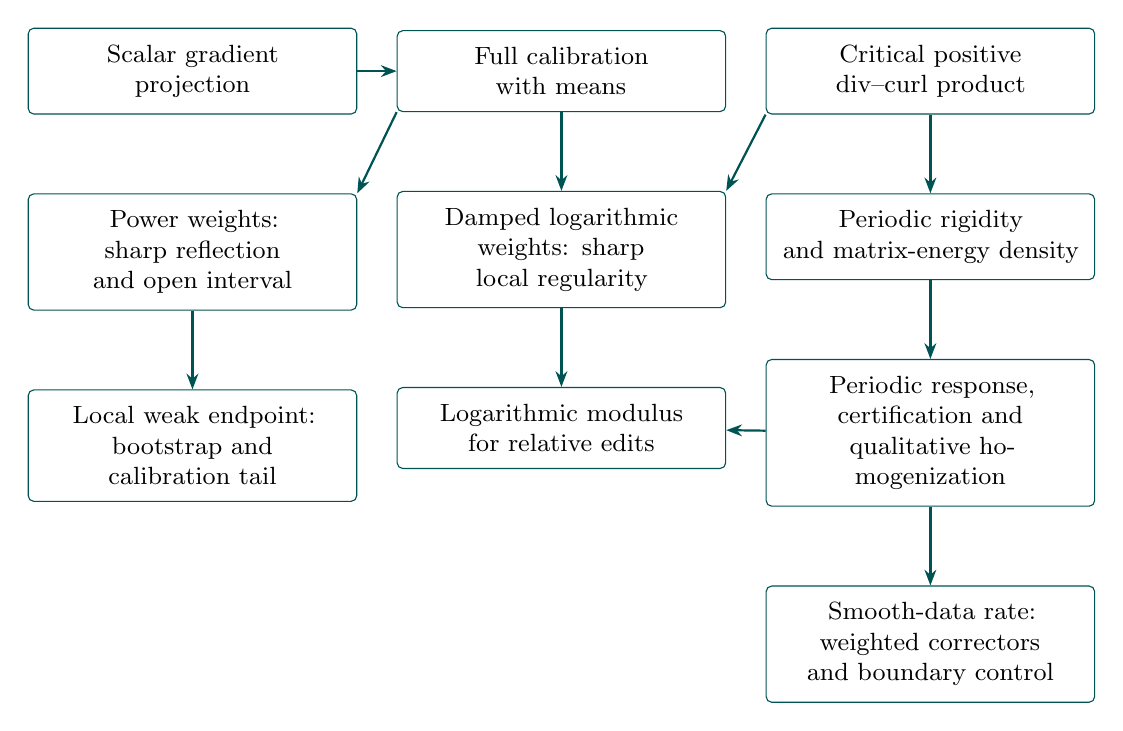
\begin{tikzpicture}[
 box/.style={draw=teal!65!black,rounded corners=2pt,align=center,
 font=\small,inner sep=6pt,text width=3.75cm},
 arr/.style={-{Stealth[length=2mm]},thick,teal!65!black},
 node distance=10mm and 5mm]
\node[box] (projection) {Scalar gradient\\projection};
\node[box,right=of projection] (calibration) {Full calibration\\with means};
\node[box,right=of calibration] (product) {Critical positive\\div--curl product};
\node[box,below=of product] (density) {Periodic rigidity\\and matrix-energy density};
\node[box,below=of projection] (power) {Power weights:\\sharp reflection\\and open interval};
\node[box,below=of calibration] (log) {Damped logarithmic\\weights: sharp\\local regularity};
\node[box,below=of power] (weak) {Local weak endpoint:\\bootstrap and\\calibration tail};
\node[box,below=of log] (stability) {Logarithmic modulus\\for relative edits};
\node[box,below=of density] (response) {Periodic response,\\certification and\\qualitative homogenization};
\node[box,below=of response] (rate) {Smooth-data rate:\\weighted correctors\\and boundary control};
\draw[arr] (projection)--(calibration);
\draw[arr] (product)--(density);
\draw[arr] (calibration.south west)--(power.north east);
\draw[arr] (calibration)--(log);
\draw[arr] (product.south west)--(log.north east);
\draw[arr] (density)--(response);
\draw[arr] (power)--(weak);
\draw[arr] (log)--(stability);
\draw[arr] (response)--(stability);
\draw[arr] (response)--(rate);
\end{tikzpicture}

% End embedded input

\caption{Three uses of the calibration. The local weak endpoint uses
ordinary \(L^2\) products; the critical positive-product theorem enters
the logarithmic and density branches. The smooth-data rate uses
weighted corrector potentials and density, independently of the
finite algorithm.}
\label{fig:dependencies}
\end{figure}

For power estimates, integrating the calibration in its threshold produces
a Burkholder-type expression. A scalar majorization then bounds the
reflection. For logarithmic estimates, the threshold weight is damped
before integration. This prevents assuming the very integrability one is
trying to prove. The leading coefficients of the two threshold integrals
are \(1/\beta\) and \(1/2\); they permit absorption precisely below
\(\beta=\tau\).

At the power endpoint, keep the calibration threshold instead of
integrating it out. The exact coefficient in the localized distortion
inequality gives a differential inequality for
\(\int(r-t)_+^2\). Subcritical bootstrap makes the cutoff errors
decay faster than its critical power. Integration yields the weak
distribution bound, although the strong endpoint still fails.

For periodic response, positivity provides a different benefit. A residual
orthogonal to all smooth admissible fields would create a positive
mean-zero div--curl pair. The critical-product theorem makes its integral
zero, so the residual vanishes. This proves density in both actual matrix
energy spaces. Compatible primal and dual approximations can then certify
the continuum response even when both \(A\) and \(A^{-1}\) are unbounded.
For the finite-scale rate, a boundary cutoff makes the first-order
corrector admissible. Weighted potential estimates control its boundary
cost, and an antisymmetric flux potential controls its residual.
Periodic density on a containing cube extends this argument to
the maximal variational domain.
\FloatBarrier


% End embedded input


% Begin embedded sections/02-calibration
\section{The calibration and the exact reflection norm}\label{sec:calibration}

\subsection{Projection onto a scalar gradient constraint}

The next argument is the ball-constrained version of
\cite[Lemma~4]{Agazzi2026}. We include the dimension-dependent details:
the admissible object is a scalar potential on \(Q\), and its gradient lies
in a Euclidean ball in \(\R^d\).

\begin{lemma}[Constrained scalar projection]\label{lem:scalar-projection}
Let \(t>0\), \(|a_0|\leq t\), and \(\eta\in W^{1,\infty}_{\per}(Q)\).
There is \(\zeta\in W^{1,\infty}_{\per}(Q)\) such that, with
\(a=a_0+\nabla\eta\) and \(z=a_0+\nabla\zeta\),
\begin{equation}\label{eq:projection-properties}
 |z|\leq t,\qquad
 z=a\ \hbox{or}\ |z|=t\quad\hbox{a.e.},\qquad
 \int_Q z\cdot(a-z)\dd\geq0.
\end{equation}
\end{lemma}

\begin{proof}
Consider the convex subset of \(L^2(Q)\)
\[
 \mathcal C=\{\xi\in W^{1,\infty}_{\per}(Q):
                         |a_0+\nabla\xi|\leq t\ \hbox{a.e.}\}.
\]
It contains constants. It is closed in \(L^2\): an \(L^2\)-convergent
sequence has uniformly bounded gradients, bounded means, and hence
uniformly bounded Lipschitz representatives. A subsequence converges
uniformly, and weak-* convergence of its gradients preserves the convex
ball constraint. The Hilbert projection \(\zeta\) of \(\eta\) therefore
exists uniquely. Put \(h=\eta-\zeta\). Its characterization is
\begin{equation}\label{eq:projection-variation}
 \int_Qh(\xi-\zeta)\dd\leq0\qquad(\xi\in\mathcal C).
\end{equation}

Write \(w=a_0\cdot x+\zeta\). On \(\{h=0\}\), the scalar Sobolev
level-set property gives \(\nabla h=0\) almost everywhere, so \(z=a\).
At a differentiability point \(x_0\) of \(w\) where \(h(x_0)>0\), suppose
\(|\nabla w(x_0)|<t\). Choose \(\delta>0\) with
\(|\nabla w(x_0)|+2\delta<t\). For a sufficiently small ball
\(B_r(x_0)\), contained in a coordinate chart of \(Q\), \(h>0\) and
\[
 |w(x_0+y)-w(x_0)-\nabla w(x_0)\cdot y|\leq\delta|y|.
\]
The cone \(c(x)=w(x_0)+\epsilon-t|x-x_0|\), with
\(0<\epsilon<\delta r\), lies below \(w\) on the boundary and above it
at \(x_0\). Replacing \(w\) by \(\max(w,c)\) in that ball changes
\(\zeta\) by the nonzero compactly supported function \((c-w)_+\).
Both gradients satisfy the ball constraint. This contradicts
\eqref{eq:projection-variation}. For \(h(x_0)<0\), use the minimum with
the upward cone \(w(x_0)-\epsilon+t|x-x_0|\).
Rademacher's theorem proves the active-set assertion almost everywhere.
This cone construction works in every dimension.

Finally \(\zeta(\cdot\pm se_i)\in\mathcal C\). Add their two
variational inequalities and change variables to obtain
\[
 \int_Q[h(x+se_i)-h(x)]
             [\zeta(x+se_i)-\zeta(x)]\dd\geq0.
\]
Divide by \(s^2\) and let \(s\to0\), using \(W^{1,2}\) difference
quotients. Summing over \(i=1,\ldots,d\) gives
\(\int_Q\nabla\zeta\cdot\nabla h\geq0\).
The constant term contributes \(a_0\cdot\int_Q\nabla h=0\), which proves
the last assertion of \eqref{eq:projection-properties}.
\end{proof}

\subsection{The full mean-sensitive inequality}

For \(a,b\in\R^d\) set
\[
 \alpha=\tfrac12|a+b|,\quad \gamma=\tfrac12|a-b|,
 r=\alpha+\gamma,\quad D=a\cdot b=\alpha^2-\gamma^2.
\]
Use \(r\) for a generic pair and \(R\) for the physical pair in
\eqref{eq:distortion-notation}. Define
\begin{equation}\label{eq:calibration}
 L_t(a,b)=
 \begin{cases}
 D,&r\leq t,\\
 2t\alpha-t^2,&r>t.
 \end{cases}
\end{equation}
The definitions agree at \(r=t\).

\begin{lemma}[Algebraic support formula]\label{lem:support}
Let \(Z_t(a)=\{z:|z|=t\}\), augmented by \(\{a\}\) when \(|a|\leq t\).
Then
\begin{equation}\label{eq:support}
 L_t(a,b)=\sup_{z\in Z_t(a)}
              \{z\cdot b+z\cdot(a-z)\}.
\end{equation}
Moreover \(L_t\geq t|a+b|-t^2\), and \(L_t\) is globally Lipschitz
in \((a,b)\), with constant at most \(4t\).
\end{lemma}

\begin{proof}
On the sphere the supremum is \(t|a+b|-t^2\); at \(z=a\) the value is
\(D\). The comparison follows from
\[
 D-(2t\alpha-t^2)=(t-\alpha-\gamma)(t-\alpha+\gamma),
 \qquad |\alpha-\gamma|\leq|a|\leq\alpha+\gamma.
\]
These inequalities decide the maximum whenever the extra point is
admissible, and give \eqref{eq:support} in the other cases as well.
On \(r<t\), \(|a|,|b|\leq t\), so the derivatives of \(D\) are bounded
by \(t\) in each variable. On \(r>t\) the assertion follows directly
from \(t|a+b|-t^2\). Continuity across the interface gives the stated
global Lipschitz bound, by restriction to line segments.
\end{proof}

\begin{proposition}[Calibration with means]\label{prop:calibration}
If \(a=a_0+\nabla\eta\), \(\eta\in W^{1,\infty}_{\per}(Q)\), and
\(b\in L^1(Q;\R^d)\) is divergence free with mean \(b_0\), then
\begin{equation}\label{eq:mean-calibration}
 \int_QL_t(a,b)\dd\geq L_t(a_0,b_0).
\end{equation}
\end{proposition}

\begin{proof}
If \(r(a_0,b_0)>t\), Lemma~\ref{lem:support} and convexity of the norm
give the result immediately. Otherwise \(|a_0|\leq t\).
Use Lemma~\ref{lem:scalar-projection} and \eqref{eq:support}. Since
\(z\in Z_t(a)\) almost everywhere,
\[
 \int_QL_t(a,b)\dd
 \geq\int_Q z\cdot b\dd+\int_Qz\cdot(a-z)\dd
 \geq a_0\cdot b_0=L_t(a_0,b_0).
\]
For the first equality, a periodic Lipschitz potential may be tested
against an \(L^1\) divergence-free field: smooth its potential,
use uniformly bounded gradients and almost-everywhere convergence,
and apply dominated convergence. This accounts for both means.
\end{proof}

\begin{corollary}[Compact \(L^1\) version]\label{cor:compact-calibration}
If \(a,b\in L^1(\R^d;\R^d)\) have compact support,
\(\curl a=0\), and \(\diver b=0\), then
\(\int_{\R^d}L_t(a,b)\dd\geq0\).
\end{corollary}

\begin{proof}
For smooth fields, put their support inside a periodic cube.
A compactly supported curl-free field has zero mean:
write \(a=\nabla v\) and choose the potential constant off a large ball.
A compactly supported divergence-free field has zero mean because
\(\int b_i=\int\diver(x_i b)=0\).
Rescale Proposition~\ref{prop:calibration} to the cube.
For \(L^1\) fields mollify both, preserving the constraints and compact
support. The Lipschitz estimate in Lemma~\ref{lem:support} passes the
integrals to the limit. No product integrability is required for this step.
\end{proof}

\subsection{Power weights and majorization}

\begin{lemma}[Integral representation]\label{lem:burkholder}
For \(p>2\) let
\[
 \mathcal B_p(a,b)=((p-1)\gamma-\alpha)(\alpha+\gamma)^{p-1}.
\]
Then
\begin{equation}\label{eq:burkholder-rep}
 \mathcal B_p=
 \frac{p(p-1)(p-2)}2
       \int_0^\infty t^{p-3}[L_t(a,b)-D]\mathrm dt.
\end{equation}
For bounded periodic div--curl pairs,
\(\int_Q\mathcal B_p(a,b)\geq\mathcal B_p(a_0,b_0)\).
Furthermore, with \(c_p=p(1-1/p)^{p-1}\),
\begin{equation}\label{eq:majorization}
 \alpha^p-(p-1)^p\gamma^p\leq-c_p\mathcal B_p(a,b).
\end{equation}
\end{lemma}

\begin{proof}
The integrand vanishes for \(t\geq r\). Direct integration on \((0,r)\)
gives
\[
 -\frac{D r^{p-2}}{p-2}
 +\frac{2\alpha r^{p-1}}{p-1}-\frac{r^p}p.
\]
Multiplication by the coefficient in \eqref{eq:burkholder-rep} yields
the stated expression. At \(r=0\) both sides are zero.
The bound by a constant times \(r^p\) justifies integration in space
for bounded fields. Subtract the expression for the means and use
\(\int_QD=a_0\cdot b_0\) and \eqref{eq:mean-calibration}.
Although \(L_t-D\) can have either sign, the spatially integrated
difference has the required sign at every \(t\); the absolute
integrability just established permits Fubini.

For \eqref{eq:majorization}, divide by \(r^p\) if \(r>0\) and set
\(v=\gamma/r\in[0,1]\). It is enough to show
\[
 g(v)=c_p(1-pv)-(1-v)^p+(p-1)^pv^p\geq0.
\]
Here \(g(1/p)=g'(1/p)=0\), and
\[
 g''(v)=p(p-1)[(p-1)^pv^{p-2}-(1-v)^{p-2}]
\]
changes sign once, at
\(v_0=[1+(p-1)^{p/(p-2)}]^{-1}<1/p\).
On \([v_0,1]\) the function is convex and its minimum is zero.
On \([0,v_0]\) it is concave, so its minimum is at an endpoint.
The endpoint \(v_0\) is already nonnegative, while \(g(0)=c_p-1\geq0\).
For the latter fact, \(c_2=1\) and
\[
 \frac{\mathrm d}{\mathrm dp}\log c_p
 =\frac2p+\log(1-1/p)
 \geq\frac2p-\frac1{p-1}\geq0\quad(p\geq2).
\]
This proves the scalar majorization.
\end{proof}

For a real trigonometric polynomial \(f\), choose
\(a=Pf\), \(b=-(\Id-P)f\). Then \(a+b=Hf\), \(a-b=f\);
the means are \(a_0=0\), \(b_0=-\mean fQ\), so
\(\alpha_0=\gamma_0\) and \(\mathcal B_p(a_0,b_0)\geq0\).
Lemma~\ref{lem:burkholder} therefore proves
\(\norm{Hf}_p\leq(p-1)\norm f_p\) for \(p>2\).
Density extends \(H\) to \(L^p(Q)\).
For \(p=2\), \(P\) is orthogonal and \(H\) is an isometry.
The real \(L^2\) pairing makes \(H\) self-adjoint. Duality gives
\(\norm H_p=\norm H_{p'}\leq(p-1)^{-1}\) below two, and also shows
that the extensions retain \(H^2=\Id\).

\subsection{Transfer to Euclidean space}

First let \(f\) be a real Schwartz field with Fourier transform supported
in an annulus away from zero. The fields \(a=Pf\) and
\(b=-(\Id-P)f\) have Schwartz potentials
\[
 a=\nabla\phi,\qquad b_i=\sum_j\partial_j\Psi_{ij},\quad
 \Psi_{ij}=-\Psi_{ji},\qquad
 \widehat\Psi_{ij}(\xi)
 =\frac{\xi_j\widehat b_i-\xi_i\widehat b_j}{2\pi i|\xi|^2}.
\]
Let \(\chi_R(x)=\chi(x/R)\) with \(\chi=1\) near the origin.
The compact fields
\[
 a_R=\nabla(\chi_R\phi),\qquad
 (b_R)_i=\sum_j\partial_j(\chi_R\Psi_{ij})
\]
are exactly curl free and divergence free. They converge to \(a,b\)
in every \(L^p\), \(1<p<\infty\). On a periodic cube containing
their support, apply the preceding calibration, representation and
majorization with zero means. Then let \(R\to\infty\).
This proves the Euclidean upper bound on this dense class.

For completeness, annular Fourier-supported Schwartz fields are dense
in \(L^p\). Approximate first by smooth compactly supported fields;
smooth high-frequency truncation converges by the approximate-identity
theorem, while a smooth low-frequency cutoff shrunk to zero converges
to zero in \(L^p\), \(p>1\), first on such test fields by scaling and
then by its uniformly bounded convolution norm. The norm estimate
extends \(H\) to all of \(L^p(\R^d)\). Orthogonality and duality
treat the remaining exponents as on \(Q\).

\subsection{Sharpness and the order of limits}\label{subsec:reflection-sharp}

Fix \(p>2\) in the plane and let
\(U(z)=z|z|^{-2/p}\) on \(\epsilon<|z|<1\).
Choose smooth radial cutoffs, zero for \(|z|<\epsilon/2\) and
\(|z|>2\), equal to one on the displayed annulus, with the usual
scale bounds on their derivatives. Denote the resulting smooth
compactly supported map by \(U_\epsilon=u_\epsilon+iv_\epsilon\).
On the annulus,
\[
 |\partial_zU|=(1-1/p)|z|^{-2/p},\qquad
 |\partial_{\bar z}U|=p^{-1}|z|^{-2/p}.
\]
The \(p\)-th power integrals on both cutoff annuli are bounded
independently of \(\epsilon\), by rescaling at the inner annulus.
The main integrals are proportional to \(\log(1/\epsilon)\).
Consequently
\[
 \frac{\norm{\partial_zU_\epsilon}_p}
      {\norm{\partial_{\bar z}U_\epsilon}_p}\longrightarrow p-1.
\]
With \(\Rot=\left(\begin{smallmatrix}0&-1\\1&0\end{smallmatrix}\right)\),
put \(a=\nabla u_\epsilon\), \(b=-\Rot\nabla v_\epsilon\).
The elementary Cauchy--Riemann identities give
\(|a+b|=2|\partial_zU_\epsilon|\),
\(|a-b|=2|\partial_{\bar z}U_\epsilon|\).
For \(f=a-b\), exact differential constraints give \(Hf=a+b\).
This proves the lower bound in \(\R^2\) and, by placing the compact
potentials inside a periodic cell and rescaling, on \(\T^2\).

On \(\T^d\) the same fields may be independent of the last \(d-2\)
coordinates. In \(\R^d\), multiply both planar potentials by a smooth
cutoff \(\theta(x'/L)\) in the other coordinates. Use the full gradient
of the first potential and use \(-\Rot\nabla_{x_1,x_2}\) of the second
in the first two components, with the other flux components zero.
These fields still satisfy the exact differential constraints.
For fixed \(\epsilon\), their extra gradient components have
\(L^p\) norm \(O(L^{-1}L^{(d-2)/p})\), whereas the principal norms
scale as \(L^{(d-2)/p}\). Let \(L\to\infty\) first and then
\(\epsilon\to0\). This order avoids a uniform cutoff estimate
in a parameter where none is needed.
For \(p<2\), self-adjoint duality transfers the lower bound from \(p'>2\).
At \(p=2\) it is one. This proves the reflection assertion of
Theorem~\ref{thm:main-power}.

% End embedded input


% Begin embedded sections/03-ellipticity
\section{Scalar ellipticity and constitutive inversion}\label{sec:elliptic}

\subsection{A contraction principle with an error certificate}

The reflection has square equal to the identity. Thus a small Lipschitz
perturbation of it can be inverted by a fixed-point iteration. The norm
proved above determines exactly how small the perturbation must be.

\begin{theorem}[Lipschitz constitutive inversion]\label{thm:constitutive}
Let \(1<p<\infty\). Suppose \(m(x,z)\) is measurable in \(x\), continuous
in \(z\), \(m(x,0)=0\), and
\[
 |m(x,z)-m(x,w)|\leq k|z-w|
\]
almost everywhere in \(x\), for all \(z,w\in\R^d\).
If \(\vartheta=kC_p<1\), then, on \(Q\) or \(\R^d\), every \(h\in L^p\)
has a unique solution of \(Hf-m(x,f)=h\). Starting from \(f_0=0\),
\[
 f_{j+1}=H(m(x,f_j)+h)
\]
converges in \(L^p\), and
\begin{align}
 \norm f_p&\leq\frac{C_p}{1-\vartheta}\norm h_p,\label{eq:constitutive-bound}\\
 \norm{f-f_N}_p&\leq
       \frac{\vartheta^NC_p}{1-\vartheta}\norm h_p,\label{eq:picard-error}\\
 \norm{f-v}_p&\leq
       \frac{C_p}{1-\vartheta}\norm{Hv-m(x,v)-h}_p.\label{eq:residual}
\end{align}
\end{theorem}

\begin{proof}
The Nemytskii map \(f\mapsto m(\cdot,f)\) is well defined on real \(L^p\)
and has Lipschitz constant \(k\). Its composition with \(H\) is a
contraction with constant \(\vartheta\). The contraction theorem gives existence,
uniqueness and \eqref{eq:constitutive-bound}. Summing the geometric
tail of successive differences gives \eqref{eq:picard-error}.
For an arbitrary \(v\), subtract its equation from the exact one,
apply \(H\), and use \(H^2=\Id\):
\[
 \norm{f-v}_p\leq \vartheta\norm{f-v}_p+
                   C_p\norm{Hv-m(x,v)-h}_p.
\]
This proves the residual estimate, without assuming that \(v\) is an iterate.
\end{proof}

\subsection{The Cayley transformation and the zero mode}

Put
\[
 \alpha_0=\sqrt{\lambda\Lambda},\quad C=A/\alpha_0,\quad
 s=\sqrt{\Lambda/\lambda},\quad
 M=(\Id-C)(\Id+C)^{-1},\quad k=\frac{s-1}{s+1}.
\]
Symmetry and the spectral theorem give
\(\norm M_{\op}\leq k\), since the eigenvalues of \(C\) lie in
\([1/s,s]\).
Write \(G=F/\alpha_0\). If \(e=\nabla u\) has zero mean and
\(j=Ce-G\) is divergence free, define \(f=e+j\).
The Helmholtz constraints imply \(Pf=e\), \(Hf=e-j\), including at
frequency zero: \(e\) has no zero mode, whereas \(j\) may have one.
Eliminating \(e\) and \(j\) gives
\begin{equation}\label{eq:cayley}
 Hf=Mf+h,\qquad
 h=2(\Id+C)^{-1}G,\qquad e=Pf,\quad j=(\Id-P)f.
\end{equation}
Conversely, \eqref{eq:cayley} implies
\(j=Ce-G\), so this correspondence is exact in \(L^p\).
In particular no mean flux has been discarded.

For \(s>1\), \(kC_p<1\) is equivalent to both
\[
 p-1<\frac{s+1}{s-1},\qquad
 \frac1{p-1}<\frac{s+1}{s-1},
\]
which is precisely \eqref{eq:sharp-interval}. If \(s=1\), \(M=0\)
and every \(1<p<\infty\) is allowed.
Since
\[
 \norm h_p\leq\frac{2}{\lambda(s+1)}\norm F_p,\qquad
 \norm P_p\leq\frac{1+C_p}{2},
\]
Theorem~\ref{thm:constitutive} proves \eqref{eq:main-elliptic-bound}.
Poincare's inequality supplies the normalized periodic potential;
the Euclidean closed \(L^p\) gradient is a homogeneous Sobolev gradient.

At \(p=2\) the bound is \(1/\lambda\). For \(F\in L^2(Q)\), the
variational solution is the unique energy solution. If also \(F\in L^p\)
with \(p<2\), its gradient and flux lie in \(L^p\), and uniqueness in
\eqref{eq:cayley} identifies it with the constructed solution.
If \(p>2\), the constructed \(L^p\) solution lies in the energy space
and the same conclusion follows. For \(p<2\) and arbitrary \(L^p\)
data, approximate by \(L^p\cap L^2\) data; the bound proves convergence
to the bounded extension in \(W^{1,p}\). This extension, rather than an
unjustified energy identity, is the assertion for those data.

\begin{example}[An interval with visible endpoints]
For \(\lambda=1,\Lambda=9\), one has \(s=3\), \(k=1/2\).
The permitted interval is \(3/2<p<3\). At the upper endpoint the
radial example below has gradient proportional to \(r^{-2/3}\)
and an infinite \(L^3\) norm, although its energy is finite.
For a constant matrix in the same coefficient class, much more regularity
can hold. Sharpness is a uniform-class assertion.
\end{example}

\subsection{Uniformly convex scalar nonlinear equations}

\begin{theorem}[Uniformly convex integrands]\label{thm:nonlinear}
Suppose \(W(x,z)\) is measurable in \(x\), \(C^2\) in \(z\),
\(D_zW(x,0)=0\), and
\(\lambda\Id\leq D_z^2W(x,z)\leq\Lambda\Id\).
For every \(p\) in \eqref{eq:sharp-interval} and \(F\in L^p(Q;\R^d)\)
there is a unique mean-zero \(u\in W^{1,p}(Q)\) satisfying
\[
 \diver(D_zW(x,\nabla u))=\diver F.
\]
It obeys \eqref{eq:main-elliptic-bound}. The homogeneous Euclidean
assertion holds as well. This is an analytic inversion theorem;
it does not supply a finite implementation for an unrepresented
measurable integrand.
\end{theorem}

\begin{proof}
Set \(C_x(z)=D_zW(x,z)/\alpha_0\).
The map \(z\mapsto z+C_x(z)\) is globally invertible: it is the
gradient of \(|z|^2/2+W(x,z)/\alpha_0\), whose Hessian is bounded
below by \((1+1/s)\Id\). Subtracting an arbitrary linear functional
gives a coercive strictly convex function, with a unique minimizer.
Its inverse \(T_x\) is \(C^1\), with
\[
 D T_x(w)=(\Id+D C_x(T_x(w)))^{-1}.
\]
Measurability follows, for example, by minimizing on successively
finer rational grids in bounded balls and using uniqueness.
The reflected inverse
\(\mathcal R_x(w)=2T_x(w)-w\) has symmetric derivative with eigenvalues
\((1-c)/(1+c)\), \(c\in[1/s,s]\). Integrating this derivative on line
segments gives the global Lipschitz constant \(k\), and
\(\mathcal R_x(0)=0\).

For \(G=F/\alpha_0\), put
\[
 m(x,f)=\mathcal R_x(f+G)-\mathcal R_x(G),\qquad
 h=\mathcal R_x(G)+G=2T_x(G).
\]
The equation \(Hf=m(x,f)+h\) is equivalent to
\(Hf=\mathcal R_x(f+G)+G\).
Since \(Hf=2Pf-f\), this is equivalent to
\(Pf=T_x(f+G)\). Thus, with \(e=Pf\) and \(j=f-e\),
\(j=C_x(e)-G\); the exact gradient/divergence constraints prove the
desired equation. Conversely every \(W^{1,p}\) solution produces
such an \(f\), so uniqueness follows from Theorem~\ref{thm:constitutive}.
Finally \(|T_x(G)|\leq s|G|/(s+1)\); the same estimates as in
\eqref{eq:cayley} prove the bound.
\end{proof}

\subsection{Sharpness of the scalar interval}\label{subsec:elliptic-sharp}

We use the classical radial singular solution and dimensional descent
\cite[Section~5]{Meyers1963}, including the cutoff forcing needed for
the global periodic and Euclidean estimates.
Assume \(s>1\), and put \(\nu=1/s\). In a planar disk, let
\[
 A=\Lambda e_r\otimes e_r+\lambda e_\theta\otimes e_\theta,
 \qquad u_0=r^\nu\cos\theta.
\]
A polar-coordinate calculation gives
\(\diver(A\nabla u_0)=
(\Lambda\nu^2-\lambda)r^{\nu-2}\cos\theta=0\)
off the origin. More explicitly, with
\(\psi=-\Lambda\nu r^\nu\sin\theta\),
\[
 A\nabla u_0=\Rot\nabla\psi.
\]
The potentials belong to \(W^{1,2}\) near the origin, because
\(\int_0^1r^{2\nu-1}\mathrm dr<\infty\).
Their distributional derivatives therefore give the same equation
across the origin, with no point source.

Choose a smooth cutoff \(\eta\) supported inside the disk and equal
to one near zero. Set
\begin{equation}\label{eq:endpoint-forcing}
 u=\eta u_0,\qquad
 F=u_0A\nabla\eta-\psi\Rot\nabla\eta.
\end{equation}
The forcing is bounded and supported in an annulus, while
\(A\nabla u-F=\Rot\nabla(\eta\psi)\) is divergence free globally.
Extend \(A\), with the same ellipticity bounds, outside the disk.
This constructs a periodic example by putting the disk inside \(Q\),
as well as a Euclidean example.
Near the origin \(|\nabla u|\) is comparable to \(r^{\nu-1}\).
Thus its \(L^p\) norm is infinite precisely when
\[
 p\geq\frac2{1-\nu}=\frac{2s}{s-1}.
\]
The solution has finite energy, so a uniform strong upper-endpoint
estimate is impossible. Its critical tail is compatible with the
local weak endpoint proved below.

In \(Q\) of higher dimension use independence of the extra coordinates
and a block-diagonal extension of \(A\). In \(\R^d\) multiply \(u\)
and the first two components of \(F\) by an extra-coordinate cutoff.
Complete \(F\) in the remaining components by the corresponding
entries of \(A\nabla u\). They are bounded, since \(u_0\) is bounded;
the remaining flux still has only planar divergence-free components.
This gives the same local endpoint obstruction in every dimension.

For the lower endpoint, let \(T_A:F\mapsto\nabla u\) be the energy
solution operator on \(L^2\). Symmetry of \(A\) gives, for \(F,G\in L^2\),
\[
 \int_QG\cdot T_AF=\int_Q(A T_AG)\cdot T_AF
                  =\int_QF\cdot T_AG.
\]
If this operator had a uniform bounded extension on an exponent
\(p\leq2s/(s+1)\), duality would give the same bound on
\(p'\geq2s/(s-1)\), agreeing with the energy operator on the overlap.
The preceding bounded-forcing example contradicts that bound.
The same argument applies in Euclidean space. This completes
Theorem~\ref{thm:main-power}.


% Begin embedded sections/03a-weak-endpoint
\subsection{The attained local weak endpoint}\label{subsec:weak-endpoint}

Failure of a strong estimate at \(p_+=2s/(s-1)\) does not preclude
control of the distribution function at that exponent. The radial
solution above has exactly the critical power tail. To prove that every
homogeneous energy solution has at most this tail, we first gain a
strictly subcritical field moment. Its potentials then have a
supercritical moment, which makes the errors caused by localization
decay faster than the desired tail.

Only ordinary \(L^2\) products enter this argument. The critical
positive-product theorem of Section~\ref{sec:log} is unnecessary here.
Interior scalar and antisymmetric potentials are supplied by the
regularized Poincare operators
\cite[Corollary~3.4, Remark~3.5 and Proposition~4.1(i)]{CostabelMcIntosh2010}:
on a fixed ball, if \(\curl E=0\), \(\diver B=0\) and
\(E,B\in L^q\), \(1<q<\infty\), one can choose
\begin{equation}\label{eq:weak-potentials}
 \nabla v=E,\qquad B_i=\sum_j\partial_j\Psi_{ij},\qquad
 \Psi_{ij}=-\Psi_{ji},\qquad
 \norm v_{W^{1,q}}+\norm\Psi_{W^{1,q}}
 \leq C(d,q)(\norm E_q+\norm B_q).
\end{equation}
Fix the mean of \(v\) and the gauge of \(\Psi\). The closed one-form
and closed \((d-1)\)-form interpretations give precisely these two
operators on a ball; there is no cohomological term or boundary inverse.

\begin{lemma}[Local subcritical bootstrap]\label{lem:local-bootstrap}
Suppose \(C\) is measurable and symmetric on \(B_4\),
\(s^{-1}\Id\leq C\leq s\Id\), \(s>1\), and
\[
 E=\nabla u,\qquad B=CE,\qquad \diver B=0,\qquad u\in W^{1,2}(B_4).
\]
For each fixed \(2<p<p_+\),
\[
 \norm{(|E|^2+|B|^2)^{1/2}}_{L^p(B_3)}
 \leq C(d,s,p)\norm{(|E|^2+|B|^2)^{1/2}}_{L^2(B_4)}.
\]
\end{lemma}
\begin{proof}
Suppose first that the two fields belong to \(L^q\) on an outer
ball, with \(q\geq2\). Choose the potentials
\eqref{eq:weak-potentials} there and a smooth cutoff \(\chi\) supported
in that ball and equal to one on a smaller concentric ball. Extend
by zero the fields
\[
 a=\nabla(\chi v)=\chi E+g_a,\qquad
 b_i=\sum_j\partial_j(\chi\Psi_{ij})=\chi B_i+(g_b)_i,
 \quad g_a=v\nabla\chi,\quad (g_b)_i=\sum_j\Psi_{ij}\partial_j\chi .
\]
They are respectively curl free and divergence free, and are in
\(L^2(\R^d)\). Hence \(f=a+b\) satisfies \(Hf=a-b\).
Extend \(M=(\Id-C)(\Id+C)^{-1}\) by zero outside the outer ball.
Since \((\Id-C)=M(\Id+C)\),
\begin{equation}\label{eq:weak-local-inverse}
 Hf-Mf=(\Id-M)g_a-(\Id+M)g_b=:h,\qquad
 \norm M_\infty\leq\frac{s-1}{s+1}.
\end{equation}
Sobolev embedding gives \(h\in L^a\cap L^2\) whenever
\(2\leq a<p_+\) and \(a\leq dq/(d-q)\) if \(q<d\);
every finite \(a<p_+\) is available if \(q\geq d\).
At \(q=d\) only finite exponents are used.

Theorem~\ref{thm:constitutive} inverts \eqref{eq:weak-local-inverse}
in both \(L^2\) and \(L^a\). These inverses agree on the overlap:
their identical Neumann partial sums converge in both spaces, and
therefore to the same distribution. Thus the existing \(f\) belongs
to \(L^a\), with a bound by the outer \(L^q\) norms.
On \(\chi=1\), the identities \(E=(f+Hf)/2\) and
\(B=(f-Hf)/2\) give the improved field bound.

Starting at \(q=2\), use finitely many nested balls between \(B_4\)
and \(B_3\). While \(q<d\), reduce \(1/q\) at each step by
\(1/(2d)\), or by the smaller amount that reaches the prescribed
\(1/p\). Such a step stays strictly within the Sobolev range.
Once \(q\geq d\), reach \(p\) in the next step.
Stop upon reaching \(p\), so every inversion exponent remains
strictly below \(p_+\). This takes finitely many steps depending
only on \(d,p\). Choose equally spaced intermediate radii for that
number of steps. The potential, cutoff and inverse bounds then
give the stated constant. No bound uniform as \(p\uparrow p_+\)
is asserted.
\end{proof}

\begin{lemma}[Exponents for the cutoff errors]\label{lem:weak-exponents}
For \(p_+>2\), put
\[
 a=p_++\frac{p_+^2}{2(d+p_+)},\qquad
 p=\frac12\left[p_++\max\left\{
 2,\frac{da}{d+a},\frac{a(p_+-1)}{a-1},
                    \frac{a(p_+-2)}{a-2}\right\}\right].
\]
Then \(2<p<p_+<a<\infty\), \(W^{1,p}(B_3)\hookrightarrow L^a(B_3)\),
and
\begin{equation}\label{eq:weak-tail-exponents}
 \theta_1=p(1-1/a)-1>p_+-2,\qquad
 \theta_2=p(1-2/a)>p_+-2.
\end{equation}
\end{lemma}
\begin{proof}
All four entries in the maximum are strictly below \(p_+\).
For \(da/(d+a)\) this is immediate if \(d\leq p_+\). If
\(d>p_+\), substitute the formula for \(a\) into
\(a(d-p_+)<dp_+\). The two remaining inequalities follow from
\(a>p_+\) by clearing their positive denominators.
The strict inequality \(p>da/(d+a)\) gives the asserted Sobolev
embedding, including the cases \(p\geq d\). The last two entries
in the maximum are exactly the conditions in
\eqref{eq:weak-tail-exponents}.
\end{proof}

\begin{proof}[Proof of Theorem~\ref{thm:main-weak}]
Translate and dilate to \(B_4\), using
\(\widetilde u(y)=r^{-1}u(x_0+ry)\), and suppress the tilde.
Set
\[
 \begin{gathered}
 C=A/\sqrt{\lambda\Lambda},\qquad E=\nabla u,\qquad B=CE,\\
 V=(|E|^2+|B|^2)^{1/2},\qquad J=E\cdot B,\qquad
 R=(|E+B|+|E-B|)/2 .
 \end{gathered}
\]
The eigenvalues of \(C\) lie in \([1/s,s]\).
The identity \(R^2/J+J/R^2=V^2/J\), or its direct algebraic
interpretation when a field vanishes, and
\(1+c^2\leq(s+s^{-1})c\) for these eigenvalues show that
\begin{equation}\label{eq:weak-distortion}
 R^2\leq sJ,\qquad |E|,|B|\leq R\leq V
                 \leq\sqrt{1+s^2}\,|E|.
\end{equation}
For completeness, if \(\alpha=|E+B|/2\) and
\(\gamma=|E-B|/2\), then \(J=\alpha^2-\gamma^2\geq0\)
and \(R=\alpha+\gamma\). Thus \(R^2/J\geq1\), and
monotonicity of \(x+x^{-1}\) on \([1,\infty)\) proves the implication.
If \(J=0\), ellipticity forces both fields to vanish.

If \(\norm V_{L^2(B_4)}=0\), there is nothing to prove.
Otherwise divide both fields by this norm.
Lemmas~\ref{lem:local-bootstrap}--\ref{lem:weak-exponents}
give \(\norm V_{L^p(B_3)}\leq C(d,s)\).
Choose potentials on \(B_3\), a cutoff \(0\leq\chi\leq1\)
equal to one on \(B_2\), and the compact fields \(a,b\) as in
\eqref{eq:weak-local-inverse}. With
\[
 r=\frac{|a+b|+|a-b|}{2},\qquad D=a\cdot b,\qquad
 G=(|g_a|^2+|g_b|^2)^{1/2},
\]
we have
\begin{equation}\label{eq:weak-cutoff-norms}
 \norm r_p+\norm G_a\leq C(d,s),\qquad
 a,b\in L^2,\qquad \int_{\R^d}D\dd=0.
\end{equation}
Indeed the potentials have their \(L^a\) bounds by Sobolev
embedding. The zero product integral follows by testing
\(\diver b=0\) against the compactly supported \(W^{1,2}\)
potential \(\chi v\), using ordinary \(L^2\) approximation.

We retain the precise distortion coefficient under localization.
The map \((a,b)\mapsto r(a,b)\) is a norm and
\(r(g_a,g_b)\leq G\). Consequently \(\chi R\leq r+G\) and
\[
 r^2\leq s\chi^2J+2rG+3G^2.
\]
To see the last bound directly, use
\(r\leq\chi R+G\), then \(\chi R\leq r+G\) in the cross term.
Moreover
\[
 D=\chi^2J+C_0,\qquad
 C_0=\chi E\cdot g_b+\chi B\cdot g_a+g_a\cdot g_b .
\]
Since \(\chi V\leq\sqrt2\,\chi R\leq\sqrt2(r+G)\),
\[
 |C_0|\leq\sqrt2\,rG+(\sqrt2+1/2)G^2.
\]
It follows that
\begin{equation}\label{eq:weak-exact-coefficient}
 D\geq\frac1s r^2-c_s(rG+G^2).
\end{equation}
Replacing \(1/s\) by a smaller coefficient would lose the endpoint.

Define the finite \(C^1\) function
\[
 F(t)=\int_{\R^d}(r-t)_+^2\dd,\qquad
 F'(t)=-2\int_{\R^d}(r-t)_+\dd,\qquad t>0.
\]
The compact calibration, Corollary~\ref{cor:compact-calibration},
and \eqref{eq:weak-cutoff-norms} imply
\[
 \int_{\{r>t\}}(r-t)(D/r-t)\dd
 =\int_{\R^d}(D-L_t(a,b))\dd\leq0.
\]
All terms are integrable by \(a,b\in L^2\).
Insert \eqref{eq:weak-exact-coefficient} and use
\((r-t)/r\leq1\). Since
\[
 \int_{\{r>t\}}(r-t)(r/s-t)\dd
 =\frac1s\left(F(t)+\frac{s-1}{2}tF'(t)\right),
\]
we obtain
\begin{equation}\label{eq:weak-ode}
 F(t)+\frac{s-1}{2}tF'(t)
 \leq C_s\int_{\{r>t\}}(rG+G^2)\dd .
\end{equation}

For \(t\geq1\), Holder and \eqref{eq:weak-cutoff-norms} give
\begin{align*}
 \int_{\{r>t\}}rG
 &\leq\norm G_a
       \left(\int_{\{r>t\}}r^{a/(a-1)}\right)^{(a-1)/a}
 \leq C t^{-\theta_1},\\
 \int_{\{r>t\}}G^2
 &\leq\norm G_a^2|\{r>t\}|^{1-2/a}
 \leq C t^{-\theta_2}.
\end{align*}
The first estimate uses \(p>a/(a-1)\); in both estimates
\(\int r^p\leq C\). Put
\(\kappa=p_+-2=2/(s-1)\) and
\(\eta=\min\{\theta_1,\theta_2\}-\kappa>0\).
Equation~\eqref{eq:weak-ode} becomes
\[
 tF'(t)+\kappa F(t)\leq C t^{-\kappa-\eta},
 \qquad (t^\kappa F(t))'\leq C t^{-1-\eta}.
\]
Integrating from \(1\) to \(t\), and using
\(F(1)\leq\norm r_2^2\leq C\), proves
\[
 F(t)\leq Ct^{-\kappa},\qquad
 |\{r>2t\}|\leq t^{-2}F(t)\leq Ct^{-p_+}\quad(t\geq1).
\]
On \(B_2\), \(r=R\), so \eqref{eq:weak-distortion} proves the
weak bounds for both fields on \(B_1\). For thresholds below \(2\)
the volume of \(B_1\) supplies the bound. Restore the field norm,
use \(\norm V_2\leq\sqrt{1+s^2}\norm E_2\), and restore the
spatial dilation. Under the chosen rescaling the gradient and
normalized flux have unchanged values at corresponding points,
whereas both a level-set measure and its ball volume acquire
the factor \(r^d\). Likewise
\(\fint_{B_4}|\nabla\widetilde u|^2
=\fint_{B_{4r}(x_0)}|\nabla u|^2\).
The fixed volumes of \(B_1,B_4\) therefore give exactly
\eqref{eq:main-weak}.
\end{proof}

\subsubsection*{Sharpness within the homogeneous class}

Use the uncut solution \(u_0=r^{1/s}\cos\theta\) from
Section~\ref{subsec:elliptic-sharp}, on the entire planar \(B_4\).
It solves the homogeneous equation, including at zero, and has finite
energy. Since
\[
 s^{-1}r^{1/s-1}\leq|\nabla u_0|\leq r^{1/s-1},
\]
its distribution on \(B_1\), for all sufficiently large \(t\),
satisfies
\[
 c_s t^{-p_+}\leq
 |\{x\in B_1:|\nabla u_0|>t\}|\leq C_s t^{-p_+}.
\]
The normalized flux has the same comparison, by ellipticity.
In dimension \(d>2\), take independence of the remaining coordinates
and use the block \(\lambda\Id\) there. The two-dimensional
singularity remains locally square integrable. An inner cylinder
in \(B_1\) and the containing cylinder give the same two tail
bounds by Fubini. These are homogeneous solutions on \(B_4\);
the forcing cutoff used for the global strong obstruction is absent.

Thus no weak exponent larger than \(p_+\) holds uniformly.
Nor can the endpoint be replaced by \(L^{p_+,b}\) for any finite
Lorentz index \(0<b<\infty\). In the distribution-function convention,
finiteness of this Lorentz quasinorm requires
\[
 \int_0^\infty
 \left[t\,|\{|g|>t\}\cap B_1|^{1/p_+}\right]^b\frac{\mathrm dt}{t}
 <\infty.
\]
The lower tail bound makes its integral at infinity diverge.
In particular the strong \(L^{p_+}\) endpoint fails, consistently
with the maximal open interval.

\begin{corollary}[Homogeneous uniformly convex equations]
\label{cor:nonlinear-weak}
Let \(W\) satisfy the hypotheses of Theorem~\ref{thm:nonlinear},
with \(s>1\). If \(u\in W^{1,2}(B_{4r})\) satisfies
\(\diver D_zW(x,\nabla u)=0\), then \eqref{eq:main-weak} holds
for both \(\nabla u\) and \(D_zW(x,\nabla u)/\sqrt{\lambda\Lambda}\),
with the same right-hand side and dependence \(C(d,s)\).
\end{corollary}
\begin{proof}
The measurable symmetric matrix
\[
 A_u(x)=\int_0^1D_z^2W(x,t\nabla u(x))\,\mathrm dt
\]
has the bounds \(\lambda\Id\leq A_u\leq\Lambda\Id\).
The normalization \(D_zW(x,0)=0\) gives
\(D_zW(x,\nabla u)=A_u\nabla u\).
Apply Theorem~\ref{thm:main-weak} to this existing energy solution.
The linear examples above are already uniformly convex quadratic
integrands, so they also test the sharpness of this class.
\end{proof}

% End embedded input


\subsection{A represented finite Fourier solver}

For \(m(x,z)=M(x)z\), suppose \(M,h\) are rational trigonometric
polynomials, real as fields, with a certified \(\norm M_\infty\leq k\)
and \(\vartheta=kC_p<1\). Finite convolution and the rational symbol
\eqref{eq:projection-symbol} compute every Picard iterate exactly.
If \(H_0\) is a rational upper bound for \(\norm h_p\), then the gradient
error is bounded by
\begin{equation}\label{eq:fourier-cap}
 \norm{Pf-Pf_N}_p\leq
 \frac{(1+C_p)C_p}{2(1-\vartheta)}\vartheta^NH_0.
\end{equation}
Choose \(N\) from this bound before starting. An optional residual
test uses \eqref{eq:residual}, multiplied by \((1+C_p)/2\), and a
rational Fourier-coefficient bound for the residual norm.
Such a coefficient bound need not itself tend to zero; it must not
replace the a priori iteration cap.

The concrete example reconstructed in Appendix~\ref{app:fourier} has
\(d=2,p=4,k=3/10\),
\[
 M=\frac3{10}
 \begin{pmatrix}
 \cos(2\pi x_1)&\sin(2\pi x_1)\\
 \sin(2\pi x_1)&-\cos(2\pi x_1)
 \end{pmatrix},\qquad
 h=\binom{\cos(2\pi x_2)}{\sin(2\pi(x_1+x_2))}.
\]
Exact convolution gives \(M^2=k^2\Id\), hence
\(\norm M_\infty=k\). Its coefficient and forcing are
\[
 A=\frac{(1+k^2)\Id-2M}{1-k^2},\qquad
 F=\frac{(\Id-M)h}{1-k^2}.
\]
They satisfy \(A(\Id+M)=\Id-M\) and
\(2(\Id+A)^{-1}F=h\) exactly.
The ellipticity endpoints are \(7/13,13/7\); the scalar interval is
\(13/10<p<13/3\). The accompanying script verifies the differential
constraints and an exact rational \(L^4\) error certificate.

% End embedded input


% Begin embedded sections/04-logarithmic
\section{Critical products, localization and logarithmic regularity}\label{sec:log}

\subsection{The distortion geometry and the initial integrability}

For any pair with \(J\geq0\), write
\(\alpha=|E+B|/2,\gamma=|E-B|/2\). Then
\[
 J=\alpha^2-\gamma^2,\quad R=\alpha+\gamma,\quad
 V^2=2(\alpha^2+\gamma^2),\qquad
 J\leq R^2\leq V^2\leq2R^2.
\]
If \(J>0\), put \(\kappa=R^2/J\geq1\). The identity
\(V^2/J=\kappa+\kappa^{-1}\), and monotonicity of
\(x+x^{-1}\) on \([1,\infty)\), prove
\[
 R^2\leq KJ
 \quad\Longleftrightarrow\quad
 V^2\leq(K+K^{-1})J.
\]
For \(J=0\), either inequality forces both fields to vanish.

On a finite-volume subdomain \(D\), Holder's inequality gives, for \(1<q<2\)
and \(m=q/(2-q)\),
\begin{equation}\label{eq:initial-q}
 \left(\fint_DV^q\dd\right)^{2/q}
 \leq2\mean JD\left(\mean{K^m}D\right)^{1/m}
 \leq\frac{2m}{\ee\tau}\mean JD
                     \left(\mean{\ee^{\tau K}}D\right)^{1/m}.
\end{equation}
The last step uses
\(t^m\leq(m/(\ee\tau))^m\ee^{\tau t}\).
This proves every subquadratic local field moment before any weak
integration by parts is used.
There is also the critical estimate
\begin{equation}\label{eq:critical-start}
 \frac{R^2}{\log(\ee+R)}
 \leq\frac2\tau J+\ee^{\tau K}.
\end{equation}
Indeed, on \(K\leq(2/\tau)\log(\ee+R)\) use distortion.
On the complement, \(\ee^{\tau K}>(\ee+R)^2\).
Thus \(E\) and \(B\) belong locally to the Zygmund class denoted here by
\(L^2\log^{-1}L\):
\[
 F\in L^2\log^{-1}L(D)
 \quad\hbox{means}\quad
 \int_D\frac{|F|^2}{\log(\ee+|F|)}\dd<\infty.
\]
Changing the positive constant inside the logarithm gives the same class.

\subsection{The imported critical-product theorem}

We state the precise working version of the critical positive-product
result used below. It is the \(p=2\) nonnegative case of
Sbordone \cite[Corollary~3.3 and the following discussion,
p.~745]{Sbordone1997}. Positivity is part of the import; a formal
div--curl identity for arbitrary subquadratic fields is not being assumed.

\begin{theorem}[Positive critical div--curl product]\label{thm:critical-product}
Let \(U,W\in L^2\log^{-1}L_{\loc}(D;\R^d)\), with
\(\curl U=0\), \(\diver W=0\). Suppose their pointwise scalar product
is nonnegative and locally integrable. If \(u\) is a local scalar
potential of \(U\), the canonical distributional product is the
pointwise product:
\begin{equation}\label{eq:critical-product}
 \diver(uW)=U\cdot W.
\end{equation}
Here one may take \(u\in W^{1,q}_{\loc}\) for any \(q<2\) sufficiently
close to two, so that \(uW\in L^1_{\loc}\); additive constants do not
affect the distribution.
\end{theorem}

All its hypotheses hold for the pair in Theorem~\ref{thm:main-log}:
\eqref{eq:critical-start} gives the two critical classes, and \(J\geq0\)
and \(J\in L^1_{\loc}\) are explicit assumptions.
For \(q=2-1/(d+1)\), the Sobolev exponent \(q^*=dq/(d-q)\) satisfies
\[
 q^*>2,\qquad \frac1q+\frac1{q^*}<1.
\]
Thus the canonical expression is concretely an \(L^1\) vector field
inside a divergence. This also specifies the convention in
\eqref{eq:critical-product}; it is not an unspecified limiting product.

\subsection{Constraint-preserving localization}\label{subsec:localization}

By a dilation and by dividing both fields by \(A_0\), it is enough to work
on \(B_2\), with
\[
 \mean{\ee^{\tau K}}{B_2}=M_0,\qquad
 \left(\mean{V^q}{B_2}\right)^{1/q}\leq1.
\]
This follows exactly from \eqref{eq:initial-q} with \(m=2d+1\).
The zero-energy case was already settled by distortion.

We use the following standard consequence of regularized Poincare
operators \cite[Corollary~3.4, Remark~3.5 and
Proposition~4.1(i)]{CostabelMcIntosh2010}.
On a ball, a curl-free \(L^q\) vector field has a scalar potential \(u\),
and a divergence-free \(L^q\) vector field has an antisymmetric potential
\(\Psi\), with
\begin{equation}\label{eq:potential-bounds}
 \begin{gathered}
 \nabla u=E,\qquad B_i=\sum_j\partial_j\Psi_{ij},
                       \qquad \Psi_{ij}=-\Psi_{ji},\\
 \norm u_{W^{1,q}(B_2)}+\norm\Psi_{W^{1,q}(B_2)}
                 \leq C(d,q)\norm V_{L^q(B_2)}.
 \end{gathered}
\end{equation}
For \(u\), fix a zero mean. For \(\Psi\), the regularized operator fixes
a gauge. To match the differential-form statement, apply the Poincare
operator to the closed one-form \(E\cdot\mathrm dx\), and to the
closed \((d-1)\)-form obtained from \(B\) by interior multiplication
with the volume form. A ball is starlike, so there is no cohomological
term. The operators have order \(-1\), giving \(L^q\to W^{1,q}\).
Only interior potentials are used; no boundary trace or compact-support
inverse is imported.

Let \(0\leq\chi\leq1\) be smooth, supported in \(B_2\), and equal
to one on \(B_1\). Extend the following fields by zero:
\[
 a=\nabla(\chi u)=\chi E+g_a,\qquad
 b_i=\sum_j\partial_j(\chi\Psi_{ij})=\chi B_i+(g_b)_i,
 \quad
 g_a=u\nabla\chi,\quad (g_b)_i=\sum_j\Psi_{ij}\partial_j\chi.
\]
They are compactly supported and exactly satisfy
\(\curl a=0,\diver b=0\).
Set \(G^2=|g_a|^2+|g_b|^2\).
By \eqref{eq:potential-bounds} and Sobolev embedding,
\[
 \norm{g_a}_{q^*}+\norm{g_b}_{q^*}\leq C(d).
\]
For some \(\delta=\delta(d)>0\), the identities
\begin{equation}\label{eq:localized-product}
 D=a\cdot b=J_0+C_0,\qquad J_0=\chi^2J,\qquad
 C_0=\chi E\cdot g_b+\chi B\cdot g_a+g_a\cdot g_b
\end{equation}
therefore give
\begin{equation}\label{eq:cutoff-control}
 \norm{C_0}_{1+\delta}+\norm{G^2}_{1+\delta}\leq C(d),
 \qquad \norm r_q\leq C(d),\qquad r=r(a,b).
\end{equation}
For instance take \(1+\delta\) no larger than
\(\min\{(1/q+1/q^*)^{-1},q^*/2\}\), which is strictly greater than one.

The product in \eqref{eq:localized-product} is also the canonical
product. To check this without assuming \(L^2\) fields, use
\eqref{eq:critical-product} for \(uB\), multiply by \(\chi^2\), and
apply the Sobolev product rule to the additional terms involving
\(\Psi\) and \(\chi\). Those derivatives have the integrability just
verified: \(u,\Psi,g_a,g_b\in L^{q^*}\) and
\(E,B,\nabla\Psi\in L^q\), with \(1/q+1/q^*<1\).
More explicitly, antisymmetry gives
\(\diver g_b=-B\cdot\nabla\chi\). Thus
\[
 \diver((\chi u)b)=
 \chi^2J+2\chi uB\cdot\nabla\chi+
 (\chi E+u\nabla\chi)\cdot g_b-\chi uB\cdot\nabla\chi
 =J_0+C_0.
\]
It has compact support and an \(L^1\) right-hand side. Testing with
a smooth function equal to one on that support proves
\begin{equation}\label{eq:zero-local-product}
 \int_{\R^d}D\dd=0.
\end{equation}

For every \(\eta>0\), the triangle inequality for the norm \(r(a,b)\)
and the scalar inequality \((x+y)^2\leq(1+\eta)x^2+(1+\eta^{-1})y^2\)
give
\begin{equation}\label{eq:localized-distortion}
 r^2\leq(1+\eta)KJ_0+C_\eta G^2.
\end{equation}
In addition \(r\in L^s\) for every \(s<2\), by
\eqref{eq:initial-q}, with the potential bounds at each such exponent
and a fixed choice of potentials bounded in these spaces.
The regularized operators can be chosen once and have these bounds
simultaneously. This last observation is used only to justify the
initial damped integrals.

\subsection{Damping and the two sharp coefficients}

Fix \(\beta>0\), \(0<\varepsilon<1\), and use the positive weight
\[
 w_\varepsilon(t)=t^{-1-\varepsilon}(\log t)^{\beta-1},
 \qquad t\geq\ee.
\]
Define, as zero when \(r<\ee\),
\begin{align}
 A_\varepsilon(r)&=\int_\ee^r(1-t/r)w_\varepsilon(t)\mathrm dt,
       \label{eq:A-damped}\\
 B_\varepsilon(r)&=\int_\ee^rt(r-t)w_\varepsilon(t)\mathrm dt.
       \label{eq:B-damped}
\end{align}
For \(t<r\), a direct rearrangement of \eqref{eq:calibration} gives
\[
 D-L_t=(r-t)(D/r-t).
\]
Consequently the threshold integral is
\begin{equation}\label{eq:damped-integral}
 \int_\ee^\infty(D-L_t)w_\varepsilon(t)\mathrm dt
       =D A_\varepsilon(r)-B_\varepsilon(r).
\end{equation}
This is an absolutely integrable space--threshold expression.
Indeed \(A_\varepsilon\) is bounded for fixed \(\varepsilon>0\), and
\[
 B_\varepsilon(r)\leq C_{\beta,\varepsilon}
                    (1+r^{2-\varepsilon/2}).
\]
The latter bound follows by absorbing a logarithmic power into
\(t^{\varepsilon/2}\). The initial subquadratic moments justify it
in space. Thus Fubini is valid before proving any improved moment.
Corollary~\ref{cor:compact-calibration} and
\eqref{eq:zero-local-product} imply
\begin{equation}\label{eq:integrated-damped}
 \int D A_\varepsilon(r)\dd\leq\int B_\varepsilon(r)\dd.
\end{equation}

\begin{lemma}[Uniform large-\(r\) threshold estimates]\label{lem:threshold}
Given \(\beta>0\) and \(0<\eta\leq1/8\), there are
\(0<\varepsilon_0\leq\eta/16\) and \(r_0> \ee\), depending only on
\(\beta,\eta\), such that for
\(0<\varepsilon\leq\varepsilon_0\), \(r\geq r_0\),
\begin{align}
 A_\varepsilon(r)&\geq
       \frac{1-\eta}{\beta}r^{-\varepsilon}(\log r)^\beta,
       \label{eq:A-leading}\\
 B_\varepsilon(r)&\leq
       \frac{1+\eta}{2}r^{2-\varepsilon}(\log r)^{\beta-1}.
       \label{eq:B-leading}
\end{align}
For all \(r\geq\ee\),
\(A_\varepsilon(r)\leq(\log r)^\beta/\beta\).
\end{lemma}

\begin{proof}
In \eqref{eq:A-damped}, \(t^{-\varepsilon}\geq r^{-\varepsilon}\).
Hence
\[
 A_\varepsilon(r)\geq r^{-\varepsilon}
 \left[\frac{(\log r)^\beta-1}{\beta}
       -\frac1r\int_\ee^r(\log t)^{\beta-1}\mathrm dt\right].
\]
The second term is \(o((\log r)^\beta)\), independently of
\(\varepsilon\). For \(\beta\geq1\) it is at most
\((\log r)^{\beta-1}\); for \(0<\beta<1\), split at \(\sqrt r\)
to bound it by \(r^{-1/2}+2(\log r)^{\beta-1}\).
Choosing \(r_0\) large proves \eqref{eq:A-leading}.
The upper bound follows by dropping \(1-t/r\) and \(t^{-\varepsilon}\).

For \(B_\varepsilon\), substitute \(t=rv\). If \(\beta\geq1\),
\[
 B_\varepsilon(r)\leq
 r^{2-\varepsilon}(\log r)^{\beta-1}
 \int_0^1(1-v)v^{-\varepsilon}\mathrm dv,
 \qquad
 \int_0^1(1-v)v^{-\varepsilon}\mathrm dv
 =\frac1{(1-\varepsilon)(2-\varepsilon)}.
\]
Choose \(\varepsilon_0\) small enough to make the last factor at most
\((1+\eta)/2\).
For \(0<\beta<1\), choose \(0<\delta_0<1/2\) such that
\((1-\delta_0)^{\beta-1}\leq1+\eta/4\).
On \(t\geq r^{1-\delta_0}\) the same integral is multiplied by at
most \(1+\eta/4\). Choose \(\varepsilon_0\leq1/4\) so that its
factor is at most \((1+\eta/4)/2\).
The omitted interval contributes, relative to
\(r^{2-\varepsilon}(\log r)^{\beta-1}\), at most
\[
 \frac{r^{-\delta_0(1-\varepsilon)}}{1-\varepsilon}
                     (\log r)^{1-\beta},
\]
which tends uniformly to zero for the chosen \(\varepsilon\).
Increase \(r_0\) until it is at most \(\eta/8\).
Since \((1+\eta/4)^2/2+\eta/8\leq(1+\eta)/2\) for
\(0<\eta\leq1/8\), this proves \eqref{eq:B-leading}.
Every threshold choice can be made using the displayed elementary
inequalities; no limit is taken in \(\varepsilon\) here.
\end{proof}

\subsection{Absorption exactly below the exponential threshold}

Now fix \(0<\beta<\tau\), and choose
\[
 \sigma=\frac{\beta+\tau}{2},\qquad
 \eta=\frac{\sigma-\beta}{8\sigma},\qquad
 a_*=\frac{1-\eta}{\beta},\qquad b_*=\frac{1+\eta}{2}.
\]
These choices satisfy
\begin{equation}\label{eq:absorption-margin}
 c_*:=a_*-\frac{2b_*(1+\eta)}{\sigma}
 \geq\frac{\sigma-\beta}{2\beta\sigma}>0.
\end{equation}
Indeed, with \(x=\beta/\sigma\in(0,1)\),
the numerator after multiplication by \(\beta\) is
\(1-\eta-x(1+\eta)^2\geq1-x-3\eta-\eta^2
\geq(1-x)/2\), because \(\eta=(1-x)/8\).

Let
\[
 X_\varepsilon=\int_{\{r\geq r_0\}}
 J_0r^{-\varepsilon}(\log r)^\beta\dd,\qquad
 Y_\varepsilon=\int_{\{r\geq r_0\}}
 r^{2-\varepsilon}(\log r)^{\beta-1}\dd.
\]
Equations \eqref{eq:localized-product} and
\eqref{eq:integrated-damped}, followed by Lemma~\ref{lem:threshold}, give
\begin{equation}\label{eq:XY-first}
 a_*X_\varepsilon\leq b_*Y_\varepsilon+C(d,\beta,\tau).
\end{equation}
Here is the uniform error accounting. Since \(D\leq r^2\) and
\(J_0=D-C_0\geq0\), the part with \(r<r_0\) is bounded by a constant
and \(\int|C_0|\). Also
\[
 \int |C_0|A_\varepsilon(r)
 \leq\frac1\beta\int |C_0|\log^\beta(\ee+r)\leq C(d,\beta),
\]
using \eqref{eq:cutoff-control}, Holder, and
\(\log^a(\ee+r)\leq C_{a,b}(1+r^b)\) for any \(a,b>0\).
The small-\(r\) contribution of \(B_\varepsilon\) is uniformly bounded
by its undamped integral on a finite threshold interval. The same
argument controls every integral of
\(G^2\log^a(\ee+r)\), uniformly in \(\varepsilon\).

On the set \(K\leq2\log r/\sigma\), use
\eqref{eq:localized-distortion} to obtain
\[
 r^{2-\varepsilon}(\log r)^{\beta-1}
 \leq\frac{2(1+\eta)}{\sigma}
       J_0r^{-\varepsilon}(\log r)^\beta
       +C_\eta G^2r^{-\varepsilon}(\log r)^{\beta-1}.
\]
No extra power of the distortion remains.
On the complement \(r^2<\ee^{\sigma K}\);
any positive logarithmic power is bounded by a polynomial in \(K\),
which is absorbed into \(\ee^{(\tau-\sigma)K}\). Thus
\begin{equation}\label{eq:XY-second}
 Y_\varepsilon\leq\frac{2(1+\eta)}{\sigma}X_\varepsilon
                         +C(d,\beta,\tau)(1+M_0).
\end{equation}
The factor \(r^{-\varepsilon}\leq1\) creates no new error since
\(r\geq r_0>\ee\).
Combine \eqref{eq:XY-first}--\eqref{eq:XY-second} and
\eqref{eq:absorption-margin} to bound both \(X_\varepsilon\) and
\(Y_\varepsilon\) by \(C(d,\beta,\tau)(1+M_0)\), independently of
\(0<\varepsilon\leq\varepsilon_0\).

As \(\varepsilon\downarrow0\), their nonnegative integrands increase.
Monotone convergence therefore gives the undamped estimates. On \(B_1\),
\(\chi=1\), \(g_a=g_b=0\), so \(r=R\) and \(J_0=J\).
The inequalities \(J\leq R^2\), \(R^2\leq V^2\leq2R^2\) compare
the logarithms above and below, including when \(\beta-1<0\).
The bounded region \(R<r_0\) contributes a constant. This proves
the normalized estimate \eqref{eq:normalized-log} after undoing the
two normalizations. Covering compact subsets proves
\eqref{eq:log-conclusions}. No undamped Fubini step was used.

\begin{corollary}[Energy concentration modulus]\label{cor:energy-modulus}
With the normalization of Theorem~\ref{thm:main-log}, for a measurable
\(S\subset B_r\), \(v=|S|/|B_r|\in(0,1]\), and \(0<\beta<\tau\),
\[
 \frac1{|B_r|}\int_S\frac J{A_0^2}\dd
 \leq \frac{C(d,\beta,\tau)(1+M_0)}
                    {\log^\beta(\ee+1/v)}.
\]
In particular these normalized energies are uniformly integrable
when \(M_0\) is bounded. If \(1<\beta<\tau\), the same conclusion
holds for \(V^2/A_0^2\), with logarithmic exponent \(\beta-1\).
\end{corollary}
\begin{proof}
Split \(J/A_0^2\) at \(v^{-1/2}\). The lower part contributes at most
\(\sqrt v\); bound the upper part by \eqref{eq:normalized-log} divided
by \(\log^\beta(\ee+v^{-1/2})\).
These two terms are bounded by the stated expression, since
\(\sqrt v\log^\beta(\ee+1/v)\) is bounded on \((0,1]\).
For \(V^2/A_0^2\), use its logarithmic estimate in the same way,
observing that \(\log(\ee+V/A_0)\) is comparable to
\(\log(\ee+V^2/A_0^2)\). The positive exponent requires \(\beta>1\).
\end{proof}

% End embedded input


% Begin embedded sections/05-examples
\section{Endpoint examples and scalar consequences}\label{sec:examples}

The examples use a single radial construction, which also explains the
threshold. A slowly vanishing radial profile makes the energy finite.
Its logarithmic derivative determines the distortion. Choosing that
derivative at the critical scale leaves precisely the divergent integral
\(\int^\infty(\,t\log t\,)^{-1}\mathrm dt\).
This radial method has planar finite-distortion precedents
\cite{Astala2010}; it is used here to test both members of
\eqref{eq:log-conclusions}.

\subsection{A reusable radial calculation}

Work in \(0<r<\ee^{-T}\subset\R^2\), let \(t=\log(1/r)\), and choose
a positive profile \(\rho(r)\) tending to zero at the origin, with
\(\rho'(r)=h(t)\rho(r)/r\), \(0<h\leq1\).
Set
\begin{equation}\label{eq:radial-pair}
 u=\rho(r)\cos\theta,\quad v=\rho(r)\sin\theta,\quad
 E=\nabla u,\quad B=-\Rot\nabla v,\quad
 A=h^{-1}e_r\otimes e_r+h e_\theta\otimes e_\theta.
\end{equation}
In the polar frame,
\[
 E=\frac\rho r(h\cos\theta,-\sin\theta),\qquad
 B=\frac\rho r(\cos\theta,-h\sin\theta)=AE.
\]
Consequently, with \(K=h^{-1}\),
\begin{equation}\label{eq:radial-identities}
 J=\frac{h\rho^2}{r^2},\quad
 V^2=\frac{(1+h^2)\rho^2}{r^2},\quad
 R=\frac\rho r,\quad R^2=KJ.
\end{equation}
Whenever \(\rho\to0\) and the displayed gradients are locally integrable,
the definitions extend distributionally across the origin.
Indeed the boundary term in the weak derivative of either continuous
potential is bounded by \(C r\rho(r)\), which tends to zero.
Mixed distributional derivatives then prove both constraints, including
at the origin. No divergence-free assertion is inferred only from a
punctured-domain calculation.

\subsection{Failure at the logarithmic endpoint}

Fix \(\tau>0\), and take \(T\) large enough that
\[
 \rho=t^{-\tau/2}(\log t)^{-1/2},\qquad
 h=\frac{\tau+1/\log t}{2t}<1.
\]
The derivative relation and all identities in
\eqref{eq:radial-identities} follow directly.
The potentials are continuous at zero, their gradients are in \(L^1\),
and the finite energy is
\begin{equation}\label{eq:radial-energy}
 \int_{r<\ee^{-T}}J\dd
 =2\pi\int_T^\infty h\rho^2\mathrm dt
 =\pi\frac{T^{-\tau}}{\log T}.
\end{equation}
Here \((\rho^2)'(t)=-2h\rho^2\).
The exponential moment is
\begin{equation}\label{eq:radial-exp}
 \int_{r<\ee^{-T}}\ee^{\tau K}\dd
 =2\pi\int_T^\infty
          \exp\left(-\frac{2t}{\tau\log t+1}\right)\mathrm dt<\infty.
\end{equation}
For an explicit majorant, if \(T\geq\ee\), then
\(\tau\log t+1\leq(\tau+1)\sqrt t\).
With \(c=2/(\tau+1)\), the last integral is at most
\[
 4\pi\ee^{-c\sqrt T}
                  \left(\frac{\sqrt T}{c}+\frac1{c^2}\right).
\]
Since \(\log(\ee+J)\sim2t\) and \(\log(\ee+V)\sim t\),
the two endpoint integrals at \(\beta=\tau\) are each comparable,
in their tails, to
\[
 \int_T^\infty\frac{\mathrm dt}{t\log t}=\infty.
\]
For the first, \(h\sim\tau/(2t)\); for the second,
\((1+h^2)\rho^2t^{\tau-1}\sim(t\log t)^{-1}\).
This proves simultaneous failure of both endpoint assertions.

In particular, for \(\tau=1\), finite energy and
\(\ee^K\in L^1\) do not imply separate \(L^2\) integrability.
The angular integrals satisfy
\[
 \int_0^{2\pi}|E|^2\,\mathrm d\theta
 =\int_0^{2\pi}|B|^2\,\mathrm d\theta
 =\pi(1+h^2)\rho^2/r^2.
\]
Their radial integrals contain
\(\int_T^\infty(t\log t)^{-1}\mathrm dt\).
Thus this is a failure for each field, not merely their sum.

\subsection{Every exponential moment without any power gain}

Instead choose
\[
 \rho=\exp(-2\sqrt t),\qquad h=t^{-1/2},\qquad K=\sqrt t,
 \qquad T>1.
\]
The same construction gives continuous potentials, valid global
distributional constraints on the disk, and energy
\(\pi\exp(-4\sqrt T)\).
For every finite \(\sigma>0\),
\[
 \int\ee^{\sigma K}\dd
 =2\pi\int_T^\infty\exp(-2t+\sigma\sqrt t)\mathrm dt<\infty.
\]
On angular sectors of fixed positive size, either separate field has
size at least \(\rho/(2r)\). For \(p>2\), its \(p\)-moment therefore
dominates a constant times
\[
 \int_T^\infty\exp((p-2)t-2p\sqrt t)\mathrm dt=\infty.
\]
Thus even all finite exponential moments do not imply a general
\(L^{2+\delta}\) conclusion.

Both examples lift to any \(d>2\) by independence of the extra
coordinates on a cylinder and by taking \(A=\diag(A_{\rm planar},\Id)\).
The extra field components vanish. Fubini preserves every finite
moment and every divergence just proved. The singular set becomes a
codimension-two axis; the scalar potentials remain continuous there.

\subsection{Consequences for existing scalar solutions}

Let \(A\) be symmetric positive definite and satisfy, in fixed units,
\(K^{-1}\Id\leq A\leq K\Id\).
For an existing weak solution \(u\), put \(E=\nabla u\), \(B=AE\).
If \(J=E\cdot AE\) is locally integrable and \(\ee^{\tau K}\) is
locally integrable, Theorem~\ref{thm:main-log} applies. Indeed every
eigenvalue \(a\in[K^{-1},K]\) satisfies
\[
 1+a^2\leq(K+K^{-1})a,
\]
and summing in an orthonormal eigenbasis proves the distortion inequality.
If \(\tau>1\), choose \(1<\beta<\tau\) to recover local \(L^2\)
integrability of both fields. The preceding endpoint shows why
\(\tau=1\) alone is insufficient.

More generally the same conclusion holds for an existing solution of
\(\diver\mathcal A(x,\nabla u)=0\) whenever its actual pair
\((\nabla u,\mathcal A(x,\nabla u))\) has the stated integrable
nonnegative product and distortion. No general degenerate nonlinear
existence or uniqueness theorem follows from this observation.
A pointwise condition number alone is also insufficient for the
stated hypothesis: it does not control the absolute scale of \(A\)
and its inverse. Multiplying \(A\) by an arbitrary function of \(x\)
changes the divergence equation.

% End embedded input


% Begin embedded sections/06-response
\section{Degenerate periodic response and exact error identities}\label{sec:response}

Assume \eqref{eq:exp-contract} and put \(\mu=M/\tau\).
The elementary bounds
\begin{equation}\label{eq:K-moments}
 \int_QK\dd\leq\mu,\qquad
 \int_QK^r\dd\leq r!M/\tau^r\quad(r=1,2,\ldots)
\end{equation}
will suffice for all subquadratic embeddings. In particular \(\mu\geq1\).
Write
\(\norm v_A^2=\int_Qv\cdot Av\) and
\(\norm w_{A^{-1}}^2=\int_Qw\cdot A^{-1}w\).

\subsection{Positive periodic rigidity}

\begin{lemma}[Rigidity of a positive mean-zero pair]\label{lem:rigidity}
Suppose \(E=\nabla u\) is a periodic gradient of mean zero, \(B\) is
periodic and divergence free, and \(0\leq J=E\cdot B\in L^1(Q)\).
If \(R^2\leq KJ\) and \(\ee^{\tau K}\in L^1(Q)\), then \(E=B=0\)
almost everywhere.
\end{lemma}

\begin{proof}
Equations \eqref{eq:initial-q} and \eqref{eq:critical-start} apply
on the torus. The normalized periodic potential belongs to \(W^{1,q}\)
for \(q=2-1/(d+1)\), and \(uB\in L^1\).
Theorem~\ref{thm:critical-product}, applied in coordinate balls,
identifies \(J=\diver(uB)\). These local identities give the global
periodic identity, because this is a single periodic potential.
Its integral is zero. Positivity makes \(J=0\) almost everywhere,
and distortion forces \(E=B=0\).
\end{proof}

\subsection{Density in the two actual matrix energy spaces}

Define \(X_A\) to be the distributional mean-zero periodic gradients
in \(L^2(A)\). Define \(Y_{A^{-1}}\) to be the distributionally
divergence-free periodic fields in \(L^2(A^{-1})\), with arbitrary means.
They are closed Hilbert subspaces: for example
\[
 \norm g_1\leq\sqrt\mu\,\norm g_A,\qquad
 \norm g_q^2\leq
 \left(\int_QK^{q/(2-q)}\dd\right)^{(2-q)/q}\norm g_A^2
 \quad(1<q<2),
\]
and the analogous estimates hold for \(Y_{A^{-1}}\).
Thus differential constraints and means pass to limits.
A mean-zero curl-free periodic \(L^q\) field is a periodic gradient,
as follows by Fourier approximation and Poincare's inequality.

\begin{proposition}[Primal and dual energy density]\label{prop:density}
Smooth periodic gradients are dense in \(X_A\).
Smooth periodic divergence-free fields, including constants, are dense
in \(Y_{A^{-1}}\).
\end{proposition}

\begin{proof}
Let \(\mathcal H\) be the \(A\)-norm closure of smooth gradients.
For \(g\in X_A\), project onto \(\mathcal H\), writing \(g=h+r\).
The residual \(r\) is a mean-zero gradient, and its orthogonality gives
\(\diver(Ar)=0\). The pair \(E=r,B=Ar\) has nonnegative integrable
product \(r\cdot Ar\). The eigenvalue calculation in
Section~\ref{sec:examples} gives its distortion inequality with the
same \(K\). Lemma~\ref{lem:rigidity} yields \(r=0\).

For the dual statement let \(\mathcal K\) be the \(A^{-1}\)-norm
closure of smooth divergence-free fields, and let \(r\) be the
orthogonal residual of \(B\in Y_{A^{-1}}\).
Put \(E=A^{-1}r\). Orthogonality to constant test fields gives
\(\mean EQ=0\). Orthogonality to
\((\partial_j\phi)e_i-(\partial_i\phi)e_j\) gives
\(\partial_jE_i-\partial_iE_j=0\).
Thus \(E\) is a mean-zero gradient and \(r=AE\) is divergence free.
Its product is nonnegative, integrable, and satisfies the same distortion.
Lemma~\ref{lem:rigidity} again yields \(r=0\).

These are projections only in an existence proof. They are not operations
assumed available to the computational algorithm.
\end{proof}

The distinction between the matrix energy and the scalar majorant is
essential: density is proved in \(\int g\cdot Ag\), not in the generally
stronger norm \(\int K|g|^2\).
Scalar-weight density has a substantial history; for example
\cite[Theorem~4.1]{Ambrosio2015} discusses Zhikov-type
criteria. That scalar theorem is not substituted for either of the
two residual arguments above.

\begin{corollary}[Admissible pairing]\label{cor:pairing}
If \(E=\evec+g\), \(g\in X_A\), and \(B\in Y_{A^{-1}}\), then
\[
 \int_QE\cdot B\dd=\evec\cdot\mean BQ.
\]
\end{corollary}
\begin{proof}
The product is integrable by weighted Cauchy--Schwarz.
Approximate \(g\) by smooth gradients in \(L^2(A)\);
their pairing with \(B\) is zero and passes to the limit.
\end{proof}

\subsection{Solvability among all finite-energy weak solutions}

For bounded \(F\), both constants and \(F\) have finite energies
in the appropriate spaces, by \eqref{eq:K-moments}.
On \(\evec+X_A\) minimize
\[
 \cP(E)=\int_Q(E\cdot AE-2F\cdot E)\dd.
\]
The linear term is continuous by
\(\left|\int F\cdot g\right|\leq\norm F_{A^{-1}}\norm g_A\).
Completing the square in this Hilbert affine space gives a unique
minimizer \(E_*\).
Its Euler equation against smooth gradients gives
\[
 B_*=AE_*-F,\qquad \diver B_*=0,\qquad
 B_*\in Y_{A^{-1}}.
\]
The embeddings above and Poincare give
\(E_*=\evec+\nabla u_*\), with normalized
\(u_*\in W^{1,q}\) for every \(1<q<2\).

If another finite-energy weak solution exists, the difference of its
gradient and \(E_*\) lies in \(X_A\), and its \(A\)-flux is divergence
free. Lemma~\ref{lem:rigidity} eliminates the difference.
This proves uniqueness in the maximal finite-energy weak class, not
only in the completion first used for existence. It proves the
analytic response assertion of Theorem~\ref{thm:main-response}.

\subsection{The hypercircle identity with all pairings justified}

For admissible \(E\in\evec+X_A\) and \(B\in Y_{A^{-1}}\) define
\[
 \cD(B)=2\evec\cdot\mean BQ
           -\int_Q(B+F)\cdot A^{-1}(B+F)\dd.
\]
This is the classical primal--dual or hypercircle mechanism
\cite{PragerSynge1947,Vondrejc2015}. Its novelty is not claimed here.
We derive its working identity to specify precisely what degeneracy
permits.

\begin{theorem}[Exact primal--dual error]\label{thm:hypercircle}
For every such pair,
\begin{align}
 \cP(E)-\cD(B)
 &=\norm{E-E_*}_A^2+\norm{B-B_*}_{A^{-1}}^2
       \label{eq:full-gap}\\
 &=\int_Q|A^{1/2}E-A^{-1/2}(B+F)|^2\dd.\label{eq:gap-square}
\end{align}
In particular \(\cD(B)\leq\cP(E_*)\leq\cP(E)\).
\end{theorem}

\begin{proof}
Expanding \(\cP\) around \(E_*\) leaves
\(\cP(E)-\cP(E_*)=\norm{E-E_*}_A^2\).
The cross term is
\(2\int (E-E_*)\cdot(AE_*-F)=2\int(E-E_*)\cdot B_*=0\)
by Corollary~\ref{cor:pairing}.
Similarly
\[
 \cD(B_*)-\cD(B)=\norm{B-B_*}_{A^{-1}}^2,
\]
because \(A^{-1}(B_*+F)=E_*\) and
\(\int E_*\cdot(B-B_*)=\evec\cdot\mean{B-B_*}Q\).
The same pairing gives \(\cP(E_*)=\cD(B_*)\).
This proves \eqref{eq:full-gap}.
Expand the square in \eqref{eq:gap-square} and use
\(\int E\cdot B=\evec\cdot\mean BQ\) to obtain the second identity.
Every pairing is a weighted Cauchy--Schwarz pairing, justified by
Proposition~\ref{prop:density}; none assumes separate \(L^2\) fields.
\end{proof}

\subsection{A rational enclosure with coefficient uncertainty}

Suppose bounded rational compatible fields \(\widetilde E,\widetilde B\)
are given, together with rational step matrices \(S,C\) and
\[
 \int_Q\norm{A-S}_{\op}\dd\leq\eta,\qquad
 \int_Q\norm{A^{-1}-C}_{\op}\dd\leq\zeta.
\]
Use rational upper bounds \(E_\infty\geq\norm{\widetilde E}_\infty\)
and \(B_\infty\geq\norm{\widetilde B+F}_\infty\).
The quantities
\begin{align}
 U&=\int_Q(\widetilde E\cdot S\widetilde E
                        -2F\cdot\widetilde E)\dd+\eta E_\infty^2,
       \label{eq:rational-U}\\
 L&=2\evec\cdot\mean{\widetilde B}Q
     -\int_Q(\widetilde B+F)\cdot C(\widetilde B+F)\dd
     -\zeta B_\infty^2\label{eq:rational-L}
\end{align}
are rational and satisfy
\[
 L\leq\cD(\widetilde B)\leq\cP(E_*)\leq
       \cP(\widetilde E)\leq U.
\]
Hence \(U-L\leq\epsilon^2\) certifies
\begin{equation}\label{eq:certified-field}
 \norm{\widetilde E-E_*}_A^2+
 \norm{\widetilde B-B_*}_{A^{-1}}^2\leq\epsilon^2.
\end{equation}
It also gives
\[
 \norm{\widetilde E-E_*}_1^2+
 \norm{\widetilde B-B_*}_1^2\leq\mu\epsilon^2.
\]
The two different coefficient errors and their sup-norm multipliers
are indispensable. Neither approximate matrix need be positive
pointwise for these enclosure directions to be valid.
The flux in the constitutive law is \(B+F=AE\); the certified
divergence-free field is \(B\).

% End embedded input


% Begin embedded sections/07-computation
\section{Represented data and a terminating rational algorithm}\label{sec:computation}

An arbitrary measurable coefficient cannot be acquired from finitely many
point values. A computational statement therefore needs an information
contract. We use approximations in integral norm, whose errors enter the
certificate explicitly. The inverse coefficient is constructed from this
contract; it is not an additional oracle.

\subsection{The input and the finite output}

The input consists of \(d\), rational \(\tau,M>0\) satisfying
\eqref{eq:exp-contract}, rational \(\evec\in\Q^d\), bounded rational
dyadic step data \(F\), and a finite program which, for each integer
\(s\geq1\), returns an \emph{expanded} rational dyadic step matrix
\(S_s\) and a rational \(\eta_s\leq2^{-s}\) such that
\begin{equation}\label{eq:coefficient-name}
 \int_Q\norm{A-S_s}_{\op}\dd\leq\eta_s.
\end{equation}
Every box of the stated uniform grid is listed.
Symmetrizing \(S_s\) preserves the bound, so assume symmetry.
Its program runtime \(T_A(s)\), expanded output length, grid level,
dimension and coefficient bit lengths are charged.
An infinite name and its exponential-moment promise need not be decidable
by a finite verifier. The theorem is conditional on this mathematical
input contract, as is usual for a represented real input.

Given a positive rational \(\epsilon\), the output is a finite rational
description of compatible bounded fields \(\widetilde E,\widetilde B\)
and an interval \([L,U]\) satisfying \eqref{eq:rational-U}--\eqref{eq:certified-field}.
This approximates continuum fields and their energy; it is not a finite
exact encoding of an arbitrary infinite field.

\subsection{A rational inverse filter}

\begin{lemma}[Inverse name without inverse access]\label{lem:inverse-filter}
For a symmetric matrix \(S\), rational \(R\geq1\), and integer \(k\geq1\),
put
\[
 T_R(S)=(\Id+R^2S^2)^{-1},\qquad
 C_{R,k}(S)=R^2S\sum_{j=1}^kT_R(S)^j.
\]
If \(\int_Q\norm{A-S}_{\op}\leq\eta\), then
\begin{equation}\label{eq:inverse-filter-bound}
 \norm{A^{-1}-C_{R,k}(S)}_{L^1(\op)}
 \leq \frac{k(k+3)}4R^2\eta+R2^{-k}
                  +M(R+1/\tau)\ee^{-\tau R}.
\end{equation}
All operations on a rational step matrix are finite rational operations.
The estimate permits noncommuting \(A(x)\) and \(S(x)\).
\end{lemma}

\begin{proof}
The matrix \(\Id+R^2S^2\geq\Id\), even if \(S\) has negative
eigenvalues. For the positive true matrix \(A\), the finite geometric
sum gives
\[
 A^{-1}-C_{R,k}(A)=A^{-1}T_R(A)^k.
\]
On \(\{K\leq R\}\), \(A\geq R^{-1}\Id\), so its norm is at most
\(R2^{-k}\). On the complement it is at most \(K\).
The distribution bound \(|\{K>t\}|\leq M\ee^{-\tau t}\) yields
\[
 \int_{\{K>R\}}K\dd
 \leq M(R+1/\tau)\ee^{-\tau R}.
\]

Here is the perturbation argument without a commutativity assumption.
For symmetric \(X\) set \(J_\pm(X)=(X\pm iR^{-1}\Id)^{-1}\).
Their complex operator norms are at most \(R\); the resolvent identity
therefore gives
\(\norm{J_\pm(X)-J_\pm(Y)}_{\op}\leq R^2\norm{X-Y}_{\op}\).
The identities
\[
 F_R(X):=R^2X T_R(X)=\tfrac12(J_-(X)+J_+(X)),\qquad
 T_R(X)=\frac{J_-(X)-J_+(X)}{2iR}
\]
imply
\[
 \Lip(F_R)\leq R^2,\quad \Lip(T_R)\leq R,\quad
 \norm{F_R(X)}_{\op}\leq R/2,\quad
 \norm{T_R(X)}_{\op}\leq1.
\]
Use \(C_{R,k}=F_R\sum_{j=0}^{k-1}T_R^j\) and telescope each
noncommuting power difference:
\[
 \norm{C_{R,k}(X)-C_{R,k}(Y)}_{\op}
 \leq R^2\left(k+\frac12\sum_{j=0}^{k-1}j\right)
                \norm{X-Y}_{\op}
 =\frac{k(k+3)}4R^2\norm{X-Y}_{\op}.
\]
Integration and the tail estimate prove \eqref{eq:inverse-filter-bound}.
\end{proof}

An inverse name with error \(2^{-n}\) can be selected entirely rationally.
Increase an integer \(r\geq1\) until, with \(R=\max\{1,2r/\tau\}\),
\[
 M(R+1/\tau)2^{-2r}\leq2^{-n-2}.
\]
This bounds the exponential term because \(\ee\geq2\) and \(\tau R\geq2r\).
Choose \(k\geq1\) and \(s\geq1\) so that
\[
 R2^{-k}\leq2^{-n-2},\qquad
 \frac{k(k+3)}4R^2\,2^{-s}\leq2^{-n-1}.
\]
Then \(C_n=C_{R,k}(S_s)\) has the desired \(L^1\) inverse error.
For fixed \(\tau,M\), \(r,k=O(n+\log(n+1))\) and
\(s=n+O(\log(n+1))\). These are parameter estimates, not a bound on
the coefficient program or on the spatial expansion.

\subsection{Finite compatible spaces and exact assembly}

Use the periodic dyadic grid of side \(2^{-m}\), splitting each cube
into its \(d!\) Freudenthal simplices. Let \(V_m\) consist of continuous
periodic piecewise affine scalar functions, with one nodal value fixed.
The primal affine space is
\[
 \evec+\nabla V_m.
\]
The dual space consists of constant fields plus
\[
 b_i=\sum_j\partial_j\Psi_{ij},\qquad
 \Psi_{ij}=-\Psi_{ji},\quad \Psi_{ij}\in V_m.
\]
Commuting distributional derivatives give \(\diver b=0\), including
across all simplex faces. Remove linear dependencies between these
rational piecewise constant fields by exact elimination on their arrays.
The primal dimension is at most \(2^{dm}-1\), and the dual dimension
at most \(d+\tfrac12d(d-1)2^{dm}\).

The spaces are complete for approximation in the two energy norms.
Indeed, a smooth periodic gradient is uniformly approximated by the
gradient of its nodal affine interpolant. A smooth divergence-free
field has its mean plus a smooth antisymmetric periodic potential
(obtain it by the nonzero Fourier modes); interpolate that potential
instead. Uniform field error tends to zero, so its weighted energy
tends to zero because \(A,A^{-1}\in L^1\).
Combine this with Proposition~\ref{prop:density}.

On a common dyadic simplicial refinement, every field and supplied step
coefficient is constant on each simplex. Each integral in the two
quadratic objectives is therefore a finite rational sum.
For \(\widetilde E=\evec+\sum_i c_i g_i\), the primal solve is
\[
 G^{\rm p}_{ij}=\int_Qg_i\cdot S_ng_j,\qquad
 G^{\rm p}c=-r^{\rm p},\quad
 r^{\rm p}_i=\int_Qg_i\cdot(S_n\evec-F).
\]
For \(\widetilde B=\sum_i b_iw_i\), the dual solve is
\[
 G^{\rm d}_{ij}=\int_Qw_i\cdot C_nw_j,\qquad
 G^{\rm d}b=r^{\rm d},\quad
 r^{\rm d}_i=\evec\cdot\mean{w_i}Q-\int_Qw_i\cdot C_nF.
\]
Test each Gram matrix for positive definiteness by exact rational
\(LDL^T\) elimination, checking that every pivot is positive.
If it passes, the solve is finite rational elimination; no numerical
optimization oracle is involved. A zero-dimensional primal space is
allowed and requires no solve.
Rational sup-norm bounds for the fields follow, for example, by taking
the maximum of the sum of absolute component values on all simplices.

\begin{theorem}[Uniform finite algorithm]\label{thm:finite-algorithm}
On every valid input contract, the following algorithm terminates and
returns \eqref{eq:certified-field}.

At stage \(n=1,2,\ldots\), obtain \(S_n\) and construct \(C_n\) with
inverse error at most \(2^{-n}\). For each
\(0\leq m\leq\lfloor\log_2(n+1)\rfloor\), assemble the two rational
forms above. Skip a level at which either positive-definiteness test
fails. At any remaining level solve both systems, form \(L,U\) using
\eqref{eq:rational-U}--\eqref{eq:rational-L}, and stop when
\(U-L\leq\epsilon^2\).
\end{theorem}

\begin{proof}
Every finite operation at a stage is effective under the promised
coefficient name. For a fixed level \(m\), the exact Gram matrices
using \(A,A^{-1}\) are positive definite after dependencies are
removed. Their approximate entries converge, since the basis fields
are bounded and the coefficient errors tend to zero in \(L^1\).
Thus eventually both tests pass. Matrix inversion is continuous at
these fixed positive-definite matrices, so the rational trial fields
converge to the two exact Galerkin optimizers at that level. Their
sup norms remain bounded as \(n\to\infty\).

Density and Theorem~\ref{thm:hypercircle} imply that there is some
finite level \(m\) whose exact total squared Galerkin error is less
than \(\epsilon^2/4\). The schedule visits this level at all
sufficiently large stages. At those stages the optimization errors
converge to zero, as do both uncertainty terms
\(\eta_nE_\infty^2\) and \(2^{-n}B_\infty^2\).
Eventually \(U-L<\epsilon^2\). The stopping certificate is sound by
Theorem~\ref{thm:hypercircle} and the enclosure directions already
proved. This proves termination, without a uniform spatial
approximation rate.
\end{proof}

\subsection{Paid resources and verification}

Let \(N_*\) be the first successful stage discovered by this algorithm.
It is finite and instance dependent; it is not advice supplied with
the input. If \(\ell_n\) is the largest of the trial level, the forcing
grid level, and the grid levels returned for \(S_n,S_{s_n}\), a
common mesh contains
\[
 J_n=d!\,2^{d\ell_n}
\]
simplices. Those arrays are expanded; their size is not suppressed.

For precision in the complexity statement, let \(Z_n\) be the total
binary length of all raw and filtered tables, mesh coordinates,
basis arrays and input scalars used across the levels of stage \(n\),
plus \(n+k_n+r_n+s_n+1\). The added integers are counted by value,
to pay for the finite loops. A conservative implementation using
common denominators, determinant-controlled elimination and
schoolbook integer arithmetic has cost bounded by
\begin{equation}\label{eq:algorithm-cost}
 C\sum_{n=1}^{N_*}
       [T_A(n)+T_A(s_n)+(1+Z_n)^{16}].
\end{equation}
Appendix~\ref{app:bit-costs} gives the bookkeeping. Caching calls
can only reduce this upper bound.
Memory is bounded by a fixed polynomial in the largest expanded
stage data when stages are discarded after use.

The expression is deliberately in expanded data, not in the length
of a short program describing an enormous grid. Neither \(N_*\),
\(T_A\), nor those expansions have a uniform polynomial bound here.
A certificate checker can verify the finite compatible fields,
rational integrals and error allocation without replaying the search.
It remains conditional on the coefficient-name and moment promises;
it does not decide an infinite mathematical promise.

\subsection{Two information and complexity boundaries}

\begin{proposition}[Finite deterministic point access is insufficient]
\label{prop:point-access}
Finitely many adaptive point values cannot certify the effective
response of all measurable coefficients satisfying the same fixed
contract \(\tau=1/4,M=2\), even for scalar multiples of the identity.
\end{proposition}

\begin{proof}
Answer every query by \(\Id\). After any finite terminating transcript,
the coefficient equal to \(2\Id\) except at the queried points has
exactly the same answers as \(\Id\), but effective tensor \(2\Id\)
instead of \(\Id\). Both obey the stated moment bound. Thus no
certified tolerance smaller than half their separation can hold
on both inputs. This concerns finite deterministic point information,
not the integral-error representation above.

Even restricting to smooth coefficients without a supplied modulus
does not give a uniform finite-query guarantee. Put smooth dips
to \(\Id\) around the finitely many points and use \(2\Id\) elsewhere,
with total support volume \(v<1/100\). For \(A=a\Id\),
weighted Cauchy--Schwarz gives
\(A_*\geq(\int a^{-1})^{-1}\Id\geq2(1+v)^{-1}\Id\).
The response remains separated from that of \(\Id\).
\end{proof}

\begin{proposition}[A stronger succinct claim would count]\label{prop:counting}
Suppose an algorithm evaluated the effective energy in this coefficient
class in time polynomial in a succinct circuit description, dimension,
and requested precision bits. Even for \(1\leq A\leq2\), it would
compute \(\#\mathrm{SAT}\), and in particular imply \(P=NP\).
\end{proposition}

\begin{proof}
For a circuit \(C\) on \(n\) listed bits take \(d=n+1\) and
\[
 A_C(x)=\left[1+C(\mathbf1_{x_2\geq1/2},\ldots,
                         \mathbf1_{x_{n+1}\geq1/2})\right]\Id .
\]
The coefficient is independent of \(x_1\), so \(E=e_1\) is exactly
the cell gradient for mean \(e_1\). Its effective energy is
\[
 e_1\cdot A_*e_1=1+\#\mathrm{SAT}(C)/2^n.
\]
An approximation with error \(<2^{-n-2}\) recovers the integer count
by rounding after multiplying by \(2^n\).
Expansion into the \(2^n\) boxes is not polynomial in the succinct
description; our algorithm pays for it. This is a conditional
complexity implication, not an unconditional separation or a
claim about fixed dimension.
\end{proof}

% End embedded input


% Begin embedded sections/08-homogenization
\section{Effective response and periodic homogenization}
\label{sec:homogenization}

\subsection{The effective law and its finite enclosure}

Set \(F=0\), and write \(E_{\evec},B_{\evec}\) for the cell response.
Linearity and uniqueness show that both depend linearly on \(\evec\).
Define
\[
 A_*\evec=\mean{B_{\evec}}Q,\qquad
 \evec\cdot A_*\evec=\min_{E\in\evec+X_A}\int_QE\cdot AE\dd.
\]
Corollary~\ref{cor:pairing} gives
\[
 \evec\cdot A_*f=\int_QE_{\evec}\cdot AE_f\dd
              =f\cdot A_*\evec.
\]
Thus \(A_*\) is symmetric. The constant trial field gives the upper
bound below. For the lower bound, weighted Cauchy--Schwarz applied
to \(\mean EQ=\evec\) gives
\(|\evec|^2\leq\mu\int E\cdot AE\).
Consequently
\begin{equation}\label{eq:effective-bounds}
 \mu^{-1}\Id\leq A_*\leq\mu\Id.
\end{equation}

Solve the \(d\) unit-mean cell problems with individual certificate
gaps at most \(\epsilon_{\rm ten}^2/(d\mu)\).
Let \(C\) have columns the rational mean trial fluxes, and put
\(\widehat A=(C+C^T)/2\). Then
\[
 \norm{C-A_*}_{\rm F}^2
 \leq\mu\sum_{j=1}^d
       \norm{\widetilde B_j-B_{e_j}}_{A^{-1}}^2
 \leq\epsilon_{\rm ten}^2.
\]
Symmetrization is a contraction in Frobenius norm. Hence the rational
Loewner enclosure is
\begin{equation}\label{eq:tensor-enclosure}
 \widehat A-\epsilon_{\rm ten}\Id
       \leq A_*\leq\widehat A+\epsilon_{\rm ten}\Id.
\end{equation}
Every solve and acquisition cost is included.
The local logarithmic theorem applies to these now-existing homogeneous
cell solutions, with cell energy at most \(\mu|\evec|^2\).
It was not used as an existence theorem.


% Begin embedded sections/08b-stability
\subsection{Small-region relative edits}\label{subsec:response-stability}

The energy concentration estimate has a direct response consequence.
It controls changes on a small region when the two constitutive
laws remain comparable there. This is a deduction from logarithmic
regularity and the variational principle, rather than a different
construction of an effective medium.

\begin{corollary}[Relative-edit stability]\label{cor:response-stability}
Let \(A,\widetilde A\) both satisfy \eqref{eq:exp-contract}
with the same \(\tau,M\). Suppose they agree outside a measurable
\(S\subset Q\), \(|S|=v\in(0,1]\), and
\[
 \gamma^{-1}A\leq\widetilde A\leq\gamma A,\qquad \gamma\geq1.
\]
Let \(E,\widetilde E\) be their homogeneous cell gradients with
the same mean \(\evec\). For every \(0<\beta<\tau\),
\begin{align}
 \norm{\widetilde E-E}_{\widetilde A}^2
 &\leq(\gamma+\gamma^{-1}-2)\int_S E\cdot AE\dd
 \leq\frac{C(d,\beta,\tau,M,\gamma)|\evec|^2}
                     {\log^\beta(\ee+1/v)},\label{eq:edit-field}\\
 \norm{\widetilde A_*-A_*}_{\op}
 &\leq\frac{C(d,\beta,\tau,M,\gamma)}
                     {\log^\beta(\ee+1/v)}.\label{eq:edit-tensor}
\end{align}
\end{corollary}
\begin{proof}
First the concentration corollary gives the periodic estimate
\begin{equation}\label{eq:cell-concentration}
 \int_S E\cdot AE\dd
 \leq\frac{C(d,\beta,\tau,M)|\evec|^2}
                     {\log^\beta(\ee+1/v)}.
\end{equation}
Here are the uniform normalization details. For \(|\evec|=1\)
the cell energy is at most \(\mu\). Extend the fields periodically
and cover the torus by a fixed finite family of inner balls whose
concentric doubled balls lie in a bounded union of cells.
On every doubled ball both the energy and exponential-moment
averages are bounded by constants depending only on \(d,\tau,M\).
Thus the normalization \(A_0^2\) in
Theorem~\ref{thm:main-log} is bounded above uniformly.
Corollary~\ref{cor:energy-modulus} applies to each \(S\) intersected
with an inner ball. Its relative volume is at most a fixed
multiple of \(v\). For small \(v\) the logarithms are comparable;
for the remaining \(v\) use the total energy bound.
Zero-energy balls contribute nothing. Summing proves
\eqref{eq:cell-concentration} for unit mean.
Linearity and scaling give arbitrary \(\evec\), including zero.
The same argument applies to \(\widetilde A\).

Relative comparability identifies the two gradient energy spaces.
Subtract their Euler equations and test with
\(w=\widetilde E-E\), a mean-zero gradient in both spaces:
\[
 \norm w_{\widetilde A}^2
 =-\int_S w\cdot(\widetilde A-A)E\dd
 \leq\norm w_{\widetilde A}
 \left[\int_S E\cdot
       (\widetilde A-A)\widetilde A^{-1}(\widetilde A-A)E\dd
 \right]^{1/2}.
\]
For \(C=A^{-1/2}\widetilde A A^{-1/2}\), the matrix in this
last quadratic form is
\(A^{1/2}(C+C^{-1}-2\Id)A^{1/2}\).
Its middle factor is at most
\((\gamma+\gamma^{-1}-2)\Id\), since
\(\gamma^{-1}\Id\leq C\leq\gamma\Id\).
Cancellation of \(\norm w_{\widetilde A}\), with the zero case
understood, proves the first inequality in \eqref{eq:edit-field}.

The old minimizer is an admissible trial in the edited medium, so
\[
 \evec\cdot(\widetilde A_*-A_*)\evec
 \leq\int_S E\cdot(\widetilde A-A)E\dd
 \leq(\gamma-1)\int_S E\cdot AE\dd .
\]
Interchange the two coefficients for the opposite inequality.
Apply \eqref{eq:cell-concentration} to each, and take the
supremum over unit \(\evec\); symmetry gives \eqref{eq:edit-tensor}.
\end{proof}

Both moment assumptions and bounded relative comparability are
part of the conclusion's scope. A replacement with arbitrarily
large contrast on a small set is not covered. Nor does knowing
the set \(S\) supply the represented coefficient data required
by the certified algorithm.

% End embedded input


\subsection{Periodic averaging and admissible macroscopic domains}

We use the following elementary averaging fact: if \(g\in L^1(Q)\)
is periodic and \(\phi\) is continuous with compact support, then
\[
 \int\phi(x)g(x/\delta)\dd
       \longrightarrow\left(\int_Qg\right)\int\phi.
\]
One proof approximates \(g\) in \(L^1(Q)\) by trigonometric polynomials.
Periodic cell covering bounds the approximation error uniformly on
the support of \(\phi\); each nonzero Fourier mode tends to zero
by oscillatory integration. The same covering gives uniform local
\(L^1\) bounds for \(g(x/\delta)\). We also use weak-* averaging
for bounded periodic \(g\), which follows by approximation of the
macroscopic test function in \(L^1\).

Let \(\Omega\) be bounded Lipschitz and \(q=2-1/(d+1)\).
For each \(\delta>0\) there are two permitted domain conventions:
\begin{itemize}
 \item the maximal class
 \(\{u\in W^{1,q}_0(\Omega):
       \int_\Omega\nabla u\cdot A(x/\delta)\nabla u<\infty\}\);
 \item the closure of \(C_c^\infty(\Omega)\) in that gradient-energy norm.
\end{itemize}
The latter embeds in the former. The theorem asserts the same limit
for either choice, not an unproved equality of the two spaces at
each fixed \(\delta\).
Extend the energy by \(+\infty\) outside the selected domain in \(L^2(\Omega)\).

\begin{theorem}[Degenerate periodic variational homogenization]
\label{thm:homogenization}
With either domain convention,
\[
 I_\delta(u)=\int_\Omega\nabla u\cdot A(x/\delta)\nabla u\dd
 \quad\mathop{\longrightarrow}^{\Gamma,L^2}\quad
 I_0(u)=
 \begin{cases}
 \displaystyle\int_\Omega\nabla u\cdot A_*\nabla u\dd,
                           &u\in H^1_0(\Omega),\\
 +\infty,&\text{otherwise}.
 \end{cases}
\]
Bounded-energy sequences for \(\delta\downarrow0\) are precompact in
strong \(L^2(\Omega)\). For \(f\in L^2(\Omega)\), the unique minimizers
of \(I_\delta(u)-2\int_\Omega fu\) converge in \(L^2\) to the unique
minimizer with \(A_*\).
This qualitative assertion requires no smoothness of the macroscopic
solution. The additional smooth-data rate is stated separately in
Theorem~\ref{thm:quantitative}.
\end{theorem}

\begin{proof}
\emph{Coercivity and well-defined minimizers.}
Put \(m=q/(2-q)=2d+1\). Holder gives
\begin{equation}\label{eq:homogenization-coercivity}
 \norm{\nabla u}_q^2
 \leq\left(\int_\Omega K(x/\delta)^m\dd\right)^{1/m}
                       I_\delta(u).
\end{equation}
Periodic covering of a bounded box containing \(\Omega\) and
\eqref{eq:K-moments} bound the factor uniformly for \(0<\delta\leq1\).
Poincare and the compact embedding \(W^{1,q}_0\Subset L^2\)
give precompactness, because \(q>2d/(d+2)\).
For fixed \(\delta\), each domain is a closed Hilbert space in the
energy norm. For the maximal domain this follows by convergence of
gradients in the weighted Hilbert space and in \(L^q\); the zero
trace passes through \(W^{1,q}\). The loading is continuous by
\eqref{eq:homogenization-coercivity}. Strict positivity of \(A\)
and the zero trace give strict convexity and a unique minimizer.

\emph{Lower bound.}
Let \(u_\delta\to u\) in \(L^2\) with bounded energy.
Take smooth bounded periodic divergence-free fields
\(b_1,\ldots,b_d\) and \(p\in C_c^\infty(\Omega;\R^d)\), and put
\[
 b_\delta(x)=\sum_jp_j(x)b_j(x/\delta).
\]
The pointwise square inequality yields
\[
 I_\delta(u_\delta)\geq
 2\int_\Omega\nabla u_\delta\cdot b_\delta\dd
 -\int_\Omega b_\delta\cdot A(x/\delta)^{-1}b_\delta\dd.
\]
The divergence of \(b_\delta\) is
\(\sum_j\nabla p_j\cdot b_j(x/\delta)\), with no \(1/\delta\)
term. Integration by parts is legitimate for the \(W^{1,q}\)
function and this smooth bounded field.
Strong \(L^2\) convergence and bounded periodic averaging pass the
linear term to
\(-2\int u\sum_j\nabla p_j\cdot\mean{b_j}Q\).
The quadratic term averages by the \(L^1\) averaging fact, since
the \(b_j\) are bounded and \(A^{-1}\in L^1(Q)\).

Now approximate the exact cell fluxes \(B_{e_j}\) by such \(b_j\)
in \(L^2(A^{-1})\), using Proposition~\ref{prop:density}.
Their means converge by the \(L^1\) embedding, and their quadratic
matrix converges by weighted Cauchy--Schwarz:
\[
 \mean{b_j}Q\longrightarrow A_*e_j,\qquad
 \int_Qb_i\cdot A^{-1}b_j\longrightarrow(A_*)_{ij}.
\]
Thus, for every smooth compact \(p\),
\begin{equation}\label{eq:homogenization-dual}
 \liminf_{\delta\downarrow0}I_\delta(u_\delta)
 \geq2\ip{\nabla u}{A_*p}-\int_\Omega p\cdot A_*p\dd.
\end{equation}
The first pairing is initially distributional. Its bounded quadratic
dual norm and \eqref{eq:effective-bounds} imply \(\nabla u\in L^2\):
rescale any test \(p\), optimize that scalar factor, and extend the
resulting bounded linear functional by \(L^2\) duality.
Coercivity also gives \(u\in W^{1,q}_0\) by weak convergence.
Since \(u\in H^1\) and \(\Omega\) is Lipschitz, its trace is zero,
so \(u\in H^1_0\). Supremizing \eqref{eq:homogenization-dual} over
smooth \(p\), dense in \(L^2\), proves the lower bound.
If the liminf is infinite there is nothing to prove.

\emph{Recovery for smooth macroscopic functions.}
Let \(u\in C_c^\infty(\Omega)\). Choose smooth periodic scalar
corrector trials \(\phi_j\), and define
\[
 u_\delta=u+\delta\sum_j\phi_j(x/\delta)\partial_j u.
\]
These functions lie in \(C_c^\infty(\Omega)\), so are admissible
under both domain conventions, and converge to \(u\) in \(L^2\).
Their gradients are
\[
 \sum_j(e_j+\nabla\phi_j)(x/\delta)\partial_j u
       +\delta\sum_j\phi_j(x/\delta)\nabla\partial_j u.
\]
The last term has energy \(O(\delta^2)\), since the factors are
bounded and \(A\in L^1(Q)\). Its cross term tends to zero by
weighted Cauchy--Schwarz. Averaging the leading term gives the
constant quadratic form with entries
\[
 Q^\phi_{ij}=\int_Q(e_i+\nabla\phi_i)\cdot
                             A(e_j+\nabla\phi_j)\dd.
\]
By Proposition~\ref{prop:density}, choose \(\nabla\phi_j\)
converging in \(L^2(A)\) to \(E_{e_j}-e_j\).
Then \(Q^\phi\to A_*\), including the cross entries.
Choose this trial index increasingly slowly as \(\delta\to0\):
for each fixed index the averaging and remainder estimates hold
below a sufficiently small positive threshold; take a decreasing
sequence of such thresholds and use that index between successive
ones. This diagonal sequence has the required upper limit.

\emph{General recovery and minimizers.}
Approximate any \(u\in H^1_0\) by \(C_c^\infty\) in \(H^1\);
\eqref{eq:effective-bounds} gives convergence of the limit energies.
A second diagonalization gives recovery for \(u\).
Outside \(H^1_0\) the upper-limit requirement is automatic.
This proves Gamma convergence with equicoercivity.
The loading is continuous in strong \(L^2\).
Its bounded minimizing sequences have bounded energy by
\eqref{eq:homogenization-coercivity} and Young's inequality.
The lower and recovery bounds imply that every cluster point
minimizes the limit functional. Its strict convexity gives uniqueness
and hence convergence of the whole family of minimizers.
\end{proof}

This proof is a degenerate instance of classical periodic variational
homogenization \cite[Chapter~14]{BraidesDefranceschi1998}.
It does not import a uniform ellipticity assumption into
\eqref{eq:exp-contract}, or establish a stochastic or nonperiodic theorem.


% Begin embedded sections/08a-quantitative
\subsection{A finite-scale estimate for smooth macroscopic data}
\label{subsec:quantitative}

Qualitative homogenization permits arbitrary \(L^2\) loadings on a
Lipschitz domain. A rate requires more information. Here we impose
smoothness on the homogenized solution, while leaving the microscopic
coefficient in exactly the same exponential-moment class.
The first-order corrector, flux potential and boundary cutoff are
established quantitative homogenization tools. For comparison,
Griso's uniformly elliptic result
\cite[Theorem~4.1 in the cited preprint]{Griso2004} gives a
square-root-scale corrector estimate on \(C^{1,1}\) domains with
\(L^2\) data. Degenerate quantitative theory also exists in stochastic
settings, with distinct moment and ensemble assumptions
\cite[Definition~1.1 and Section~2]{BellaKniely2024}.
We prove the particular weighted estimates and variational
admissibility needed under \eqref{eq:exp-contract}; these other
theorems are not imported into this coefficient class.

Let \(\Omega\) be a bounded \(C^2\) domain and write
\[
 A_\delta(x)=A(x/\delta),\qquad
 \norm g_{A_\delta,\Omega}^2=\int_\Omega g\cdot A_\delta g\dd .
\]
Let \(E_i=e_i+\nabla\phi_i\), \(B_i=AE_i\) be the unit-mean
cell solutions, with \(\mean{\phi_i}Q=0\). Choose periodic
antisymmetric flux potentials with zero mean so that
\begin{equation}\label{eq:flux-potential}
 b_i=B_i-A_*e_i,\qquad
 \sum_k\partial_{y_k}\sigma_{i,jk}=(b_i)_j,\qquad
 \sigma_{i,jk}=-\sigma_{i,kj}.
\end{equation}
The next lemma constructs them and controls their weighted norms.
For any periodic object \(g\), abbreviate \(g^\delta(x)=g(x/\delta)\).
Choose \(\eta_\delta\in C_c^\infty(\Omega)\) with
\[
 0\leq\eta_\delta\leq1,\quad
 \eta_\delta=0\ \hbox{if }\dist(x,\partial\Omega)<\delta,\quad
 \eta_\delta=1\ \hbox{if }\dist(x,\partial\Omega)>3\delta,\quad
 |\nabla\eta_\delta|\leq C_\Omega/\delta .
\]
Such cutoffs exist for \(0<\delta\leq\delta_0(\Omega)\).

\begin{theorem}[Smooth-data square-root rate]\label{thm:quantitative}
Assume \eqref{eq:exp-contract}. Suppose
\(u_0\in C^2(\overline\Omega)\cap H^1_0(\Omega)\), and set
\[
 f=-\diver(A_*\nabla u_0).
\]
For either of the two macroscopic domain conventions in
Theorem~\ref{thm:homogenization}, let \(u_\delta\) be the unique
minimizer of \(I_\delta(u)-2\int_\Omega fu\).
Define
\begin{equation}\label{eq:quantitative-trial}
 v_\delta=u_0+\delta\eta_\delta
                  \sum_{i=1}^d\phi_i^\delta\,\partial_i u_0,
 \qquad
 \mathcal E_\delta=\sum_{i=1}^dE_i^\delta\,\partial_i u_0 .
\end{equation}
There are \(C=C(d,\tau,M,\Omega)<\infty\) and
\(0<\delta_0=\delta_0(\Omega)\leq1\), independent of the
microscopic coefficient beyond its stated moment bound, such that
for \(0<\delta\leq\delta_0\),
\begin{align}
 \norm{u_\delta-u_0}_{L^2(\Omega)}
 &\leq C\sqrt\delta\,\norm{u_0}_{W^{2,\infty}(\Omega)},
                         \label{eq:quantitative-L2}\\
 \norm{\nabla u_\delta-\nabla v_\delta}_{A_\delta,\Omega}
 +\norm{\nabla u_\delta-\mathcal E_\delta}_{A_\delta,\Omega}
 &\leq C\left(\sqrt\delta\,\norm{\nabla u_0}_\infty
                 +\delta\norm{D^2u_0}_\infty\right).
                         \label{eq:quantitative-energy}
\end{align}
The trial \(v_\delta\) belongs to both admitted domains.
No equality of these domains at a fixed \(\delta\) is assumed.
\end{theorem}

The hypothesis is on the actual macroscopic solution, not merely
on its loading: \(f\in L^2\) by itself does not supply the stated
\(C^2\) and \(W^{2,\infty}\) bounds. The corrected-gradient estimate
is in the matrix energy; it is not an unweighted \(L^2\) gradient
estimate. Neither rate is asserted optimal.

\begin{lemma}[Weighted cell potentials]\label{lem:weighted-potentials}
Put \(q=2-1/(d+1)\), \(m=2d+1\), and \(b_0=2m/(m-1)=2+1/d\).
The potentials in \eqref{eq:flux-potential} can be chosen with
\[
 \sum_i\left(\norm{\phi_i}_{W^{1,q}(Q)}
                    +\norm{\sigma_i}_{W^{1,q}(Q)}\right)
 \leq C(d,\tau,M).
\]
Moreover
\begin{equation}\label{eq:weighted-cell}
 \sum_i\int_Q
 \left[E_i\cdot AE_i+\nabla\phi_i\cdot A\nabla\phi_i
                  +K(|\phi_i|^2+|\sigma_i|^2)\right]\dd
 \leq C(d,\tau,M).
\end{equation}
\end{lemma}
\begin{proof}
The constant trial fields give
\(\int_QE_i\cdot AE_i\leq\mu=M/\tau\).
The same number is the \(A^{-1}\) energy of \(B_i\).
Weighted Holder, with exponent \(m=q/(2-q)\), therefore bounds
\(E_i,B_i\) in \(L^q\), using
\(\int K^m\leq m!M/\tau^m\).
Subtract their means and use Poincare to obtain
\(\phi_i\in W^{1,q}\) and \(b_i\in L^q\) with controlled norms.

For an explicit periodic flux potential let \(h_i\) be the mean-zero
vector solution of \(\Delta h_i=b_i\), and set
\(\sigma_{i,jk}=\partial_k(h_i)_j-\partial_j(h_i)_k\).
Fourier modes give \(\diver h_i=0\) and
\(\diver\sigma_i=b_i\), as well as antisymmetry.
The operators \(\partial_l\partial_k\Delta^{-1}\) are the
component multipliers of the gradient projection \(P\).
Their \(L^q\) bounds follow, for example, from
\(P=(\Id+H)/2\), already proved. Applied to the derivatives
of \(\sigma_i\), these bounds and Poincare prove its \(W^{1,q}\)
bound. This constructs the potential without any elliptic
regularity assumption on \(A\).

The Sobolev exponent satisfies
\[
 q^*=\frac{dq}{d-q}>b_0=\frac{2m}{m-1}.
\]
Indeed \(q=(2d+1)/(d+1)\) and
\(q^*/b_0=d^2/(d^2-d-1)>1\).
Holder consequently gives
\[
 \int_QK(|\phi_i|^2+|\sigma_i|^2)
 \leq\norm K_m\bigl(\norm{\phi_i}_{b_0}^2
                              +\norm{\sigma_i}_{b_0}^2\bigr)\leq C .
\]
Finally
\(\nabla\phi_i\cdot A\nabla\phi_i
\leq2E_i\cdot AE_i+2e_i\cdot Ae_i\).
The integral of the last term is at most \(2\mu\).
These estimates prove \eqref{eq:weighted-cell}.
\end{proof}

\begin{lemma}[Whole-cell bounds at the boundary]\label{lem:boundary-cells}
For each fixed \(c>0\), every nonnegative periodic \(g\in L^1(Q)\)
satisfies, for \(0<\delta\leq\delta_0(\Omega,c)\),
\begin{align}
 \int_\Omega g^\delta\dd&\leq C_\Omega\int_Qg\dd,
                                      \label{eq:full-cell-cover}\\
 \int_{\Omega\cap\{\dist(x,\partial\Omega)<c\delta\}}g^\delta\dd
 &\leq C_{\Omega,c}\delta\int_Qg\dd. \label{eq:strip-cell-cover}
\end{align}
\end{lemma}
\begin{proof}
Cover the integration set by all grid cubes \(\delta(z+Q)\)
that meet it. Each contributes exactly \(\delta^d\int_Qg\).
For the full domain, their disjoint union lies in a fixed bounded
neighbourhood, hence has bounded volume. For the strip, this
union lies within distance \((c+\sqrt d)\delta\) of the boundary,
on either side. A compact \(C^2\) boundary has a tubular
neighbourhood of volume at most \(C_{\Omega,c}\delta\).
Multiplying the number of covering cubes by their common cell
integral proves both statements. The proof uses an integral
over whole cells, not a pointwise bound on \(g\).
\end{proof}

\begin{lemma}[The cutoff corrector and its domain]\label{lem:cutoff-domain}
The trial in \eqref{eq:quantitative-trial} belongs to the
smooth-energy completion, and hence to the maximal domain. With
\(d_\delta=\nabla v_\delta-\mathcal E_\delta\),
\begin{align}
 d_\delta
 &= (\eta_\delta-1)\sum_i(\nabla\phi_i)^\delta\,\partial_i u_0
   +\delta\sum_i\phi_i^\delta
       (\eta_\delta\nabla\partial_i u_0+
                          \partial_i u_0\nabla\eta_\delta),
                                      \label{eq:corrector-defect}\\
 \norm{d_\delta}_{A_\delta,\Omega}
 &\leq C\left(\sqrt\delta\,\norm{\nabla u_0}_\infty
                     +\delta\norm{D^2u_0}_\infty\right),
                                      \label{eq:corrector-defect-bound}\\
 \norm{v_\delta-u_0}_2&\leq C\delta\norm{\nabla u_0}_\infty .
                                      \label{eq:corrector-L2}
\end{align}
\end{lemma}
\begin{proof}
The weak product rule gives \eqref{eq:corrector-defect}.
The first term is supported in the \(3\delta\) boundary strip.
Apply \eqref{eq:strip-cell-cover} with
\(g=\sum_i\nabla\phi_i\cdot A\nabla\phi_i\).
Its squared energy is at most
\(C\delta\norm{\nabla u_0}_\infty^2\).
For the term with \(\nabla\eta_\delta\), use the same bound
with \(g=\sum_iK|\phi_i|^2\) and
\(\delta|\nabla\eta_\delta|\leq C\).
Its squared energy obeys the same estimate.
For the remaining term use \eqref{eq:full-cell-cover};
its squared energy is at most
\(C\delta^2\norm{D^2u_0}_\infty^2\).
Lemma~\ref{lem:weighted-potentials} controls all cell integrals,
which proves \eqref{eq:corrector-defect-bound}.
The full-cell bound for \(\sum_i|\phi_i|^2\) proves
\eqref{eq:corrector-L2}.

It remains to justify the trial's variational domain.
By Proposition~\ref{prop:density}, take smooth mean-zero
periodic \(\phi_i^{(n)}\) with
\(\nabla\phi_i^{(n)}\to\nabla\phi_i\) in \(L^2(A)\).
Weighted Holder and Poincare give convergence in \(W^{1,q}\).
The embedding used above then gives convergence in \(L^{b_0}\),
and hence in \(L^2(K)\). For each fixed \(\delta\), whole-cell
covering and the bounded macroscopic multipliers in
\eqref{eq:corrector-defect} imply energy convergence of
\[
 \delta\eta_\delta\sum_i(\phi_i^{(n)})^\delta\partial_i u_0
 \quad\hbox{to}\quad
 \delta\eta_\delta\sum_i\phi_i^\delta\partial_i u_0 .
\]
Each approximant is \(C^1\) and compactly supported in \(\Omega\).
Mollification approximates its gradient uniformly, so also in
the \(A_\delta\) energy, since \(A_\delta\in L^1(\Omega)\).
It therefore belongs to the completion of \(C_c^\infty\).

The uncorrected \(u_0\) also belongs to this completion.
Cut it off at boundary distance \(h\downarrow0\).
In a boundary tube,
\(|u_0(x)|\leq C_\Omega\dist(x,\partial\Omega)
\norm{\nabla u_0}_\infty\).
Thus the error gradients are uniformly bounded and supported
in a shrinking strip. Absolute continuity of the integral of
\(K^\delta\) makes their energy tend to zero.
Each compactly supported \(C^1\) cutoff can again be mollified
with uniform gradient convergence. This proves the claimed
membership, without identifying the two domain conventions.
\end{proof}

\begin{lemma}[Flux-potential pairing in the maximal domain]
\label{lem:maximal-flux}
If \(w\in W^{1,q}_0(\Omega)\) has finite \(A_\delta\) energy,
then, for \(p_i=\partial_i u_0\),
\begin{equation}\label{eq:maximal-flux}
 \int_\Omega b_i^\delta p_i\cdot\nabla w\dd
 =-\delta\sum_{j,k}\int_\Omega
       \sigma_{i,jk}^\delta(\partial_k p_i)(\partial_j w)\dd.
\end{equation}
Both are weighted energy pairings, and the right-hand side has
absolute value at most
\(C\delta\norm{D^2u_0}_\infty\norm{\nabla w}_{A_\delta,\Omega}\).
\end{lemma}
\begin{proof}
For smooth compact \(w\), use
\((b_i^\delta)_j=\delta\sum_k\partial_k\sigma_{i,jk}^\delta\)
and integrate by parts. The terms
\(\sigma_{i,jk}^\delta p_i\partial_k\partial_jw\)
cancel by antisymmetry. Multiplication by the \(C^1\) function
\(p_i\) is justified by approximation, giving
\eqref{eq:maximal-flux}.

To pass to the maximal domain without presuming Dirichlet density,
extend \(w\) by zero to a containing cube
\(\mathcal C_\delta\) of side \(L_\delta=N\delta\), \(N\) an
integer. Choose these cubes with a fixed positive margin around
\(\overline\Omega\), and uniformly bounded side lengths.
The zero extension is periodic \(W^{1,q}\) on the cube and has
mean-zero gradient of finite energy. The coefficient \(A_\delta\)
is periodic there. After rescaling the cube to unit size, its
normalized exponential moment is at most \(M\), because the cube
contains an integer number of periods in each coordinate.
Proposition~\ref{prop:density} therefore approximates this
gradient by smooth periodic gradients in its actual matrix energy.

Extend \(p_i\) to a compactly supported \(W^{1,\infty}\) function
on the cube. The \(C^2\) boundary permits such an extension;
only existence is needed for this density passage.
Apply the smooth identity on the cube with this extension.
It is valid for a Lipschitz multiplier by mollification:
the multipliers converge uniformly, their derivatives are
uniformly bounded and converge almost everywhere, and the
weighted integrable functions below give dominated convergence.
Both sides are continuous in the gradient energy. In fact
\[
 \int_Q b_i\cdot A^{-1}b_i
 \leq2\int_QB_i\cdot A^{-1}B_i+
                         2|A_*e_i|^2\int_QK<\infty,
 \qquad \int_QK|\sigma_i|^2<\infty .
 \]
Whole-cell covering gives their counterparts on the cube.
Weighted Cauchy--Schwarz therefore passes the identity to the
zero-extended gradient. That gradient vanishes outside \(\Omega\),
so the resulting identity is \eqref{eq:maximal-flux}.

Finally apply weighted Cauchy--Schwarz on \(\Omega\) to its
right-hand side, with \(A_\delta^{-1}\leq K^\delta\Id\),
and use \eqref{eq:full-cell-cover} and
\eqref{eq:weighted-cell}. This gives the asserted bound with
the actual interior derivatives
\(\partial_kp_i=\partial_k\partial_i u_0\).
\end{proof}

\begin{proof}[Proof of Theorem~\ref{thm:quantitative}]
For every maximal-domain \(w\), ordinary zero-trace Sobolev
integration by parts against the \(C^1\) flux \(A_*\nabla u_0\)
gives
\(\int_\Omega A_*\nabla u_0\cdot\nabla w=\int_\Omega fw\).
For example approximate \(w\) in \(W^{1,q}_0\); the flux and its
divergence are bounded. The corrected gradient satisfies
\(A_\delta\mathcal E_\delta=\sum_iB_i^\delta\partial_i u_0\).
Consequently Lemmas~\ref{lem:cutoff-domain} and
\ref{lem:maximal-flux} give
\begin{align*}
 \left|\int_\Omega A_\delta\nabla v_\delta\cdot\nabla w\dd
                         -\int_\Omega fw\dd\right|
 &\leq
 \left(\norm{d_\delta}_{A_\delta,\Omega}
                   +C\delta\norm{D^2u_0}_\infty\right)
                       \norm{\nabla w}_{A_\delta,\Omega}\\
 &\leq C\left(\sqrt\delta\,\norm{\nabla u_0}_\infty
                 +\delta\norm{D^2u_0}_\infty\right)
                       \norm{\nabla w}_{A_\delta,\Omega}.
\end{align*}
The Euler equation for \(u_\delta\) holds for every test in
its chosen Hilbert domain. The trial \(v_\delta\) belongs
to either domain, so take \(w=u_\delta-v_\delta\).
Subtracting that equation bounds
\(\norm{\nabla u_\delta-\nabla v_\delta}_{A_\delta,\Omega}\)
by the final coefficient on the right. The triangle inequality
and \eqref{eq:corrector-defect-bound} prove
\eqref{eq:quantitative-energy}.

Equation~\eqref{eq:homogenization-coercivity}, periodic
\(m\)-moment covering, Poincare and
\(W^{1,q}_0(\Omega)\hookrightarrow L^2(\Omega)\) give
\[
 \norm{u_\delta-v_\delta}_2
 \leq C(d,\tau,M,\Omega)
              \norm{\nabla u_\delta-\nabla v_\delta}_{A_\delta,\Omega}.
\]
Combine this with \eqref{eq:corrector-L2} and \(\delta\leq1\)
to obtain \eqref{eq:quantitative-L2}.
\end{proof}

% End embedded input


\subsection{An infinite laminate outside \texorpdfstring{\(A_2\)}{A2}}

On \(Q\) in dimension two, set
\[
 I_j=(2^{-j},2^{1-j}],\quad
 a(x_1)=
 \begin{cases}j,&x_1\in I_j,\ j\ {\rm odd},\\
               1/j,&x_1\in I_j,\ j\ {\rm even},\end{cases}
 \qquad A(x)=a(x_1)\Id .
\]
Null-set values at endpoints may be assigned arbitrarily.
Both \(A\) and \(A^{-1}\) are essentially unbounded.
Here \(K=j\) on \(I_j\), so
\[
 \int_Q\ee^{K/4}\dd=\sum_{j\geq1}2^{-j}\ee^{j/4}<2.
\]
Indeed \(\ee^{1/4}<4/3\), for example by integrating \(1/x\) on
\([1,4/3]\). Thus \(\tau=1/4,M=2,\mu=8\) is a valid rational contract.
At an interface between odd \(j\) and even \(j+1\), a sufficiently
small centered ball has equal halves with values \(j\) and \(1/(j+1)\).
Its product of the averages of \(a\) and \(a^{-1}\) is at least
\(j(j+1)/4\). Hence this scalar weight is not Muckenhoupt \(A_2\).

Let \(a_J\) agree with \(a\) on the first \(J\) strips and equal one
on the remaining tail. The explicit coefficient-name error is
\[
 \int_Q|a-a_J|\dd\leq\sum_{j>J}(j+1)2^{-j}=(J+3)2^{-J}.
\]
Choosing \(J\) by a rational stopping test gives
\eqref{eq:coefficient-name}. Expanding it onto a uniform dyadic
grid is expensive and is charged in the universal algorithm.
For this special example, a separate finite certificate integrates
the explicitly listed strips directly, paying \(O(J)\) strip data
instead of pretending to expand a huge grid.

For mean \(e_1\), \(E=(h/a,0)\), \(B=(h,0)\),
\(h=(\int_Qa^{-1})^{-1}\).
For mean \(e_2\), \(E=(0,1)\), \(B=(0,a)\).
The constraints and finite energies are immediate, and uniqueness
identifies these as the cell solutions. Their means give
\begin{equation}\label{eq:laminate-effective}
 A_*=\diag\left(
  \frac1{8/9+\tfrac12\log3},
  \frac{10}{9}+\tfrac12\log(4/3)\right).
\end{equation}
For clarity, the even integer sum is
\(\sum_{k\geq1}2k\,4^{-k}=8/9\), and the odd one is \(10/9\).
The reciprocal odd sum is
\(\sum_{j\ {\rm odd}}2^{-j}/j=\tfrac12\log3\), while the
reciprocal even sum is \(\tfrac12\log(4/3)\).
These follow from the geometric series and
\(\sum_{k\geq1}z^k/k=-\log(1-z)\), obtained by integration on
\(|z|<1\). Formula \eqref{eq:laminate-effective} is an identity for
comparison, not a numerical logarithm oracle.

\subsection{Finite rational laminate trials}

Put \(t_J=2^{-J}\), \(h_J=(\int_Qa_J^{-1})^{-1}\), and take
\[
 \widetilde E_1=(h_J/a_J,0),\quad\widetilde B_1=(h_J,0),\qquad
 \widetilde E_2=(0,1),\quad\widetilde B_2=(0,a_J).
\]
Their means and differential constraints are exact.
Let \(O_J,N_J\) be respectively the odd and even integer tails
\(\sum_{j>J,\ {\rm parity}}j2^{-j}\); let \(w_o,w_e\) be their
corresponding strip volumes. All four are rational geometric sums.
Then rational upper bounds for the two true tails are
\[
 a_{\rm tail}\leq U_a:=O_J+\frac{w_e}{J+1},\qquad
 (a^{-1})_{\rm tail}\leq U_b:=N_J+\frac{w_o}{J+1}.
\]
Writing \(a_{\rm pre}=\sum_{j\leq J}2^{-j}a_j\), primal--dual
evaluation yields
\begin{align*}
 L_1&=h_J-h_J^2(U_b-t_J),&
 U_1&=h_J+h_J^2(U_a-t_J),\\
 L_2&=a_{\rm pre}+2t_J-U_b,&
 U_2&=a_{\rm pre}+U_a.
\end{align*}
These enclose the two exact minimum energies. Their widths are exactly
\begin{equation}\label{eq:laminate-gap}
 U_1-L_1=h_J^2T_J,\qquad U_2-L_2=T_J,\qquad
 T_J=\left[J+\frac1{J+1}\right]2^{-J}.
\end{equation}
Indeed \(O_J+N_J=(J+2)2^{-J}\) and \(w_o+w_e=t_J\).
This also proves the bound for the full tail mismatch
\(\sum_{j>J}2^{-j}(a_j+a_j^{-1}-2)\).

The supplied new script evaluates these fractions at \(J=50\),
without logarithms or floating-point decisions.
The widths are less than \(2.148\cdot10^{-14}\) and
\(4.443\cdot10^{-14}\), respectively. Their sum, multiplied by
\(\mu=8\), is less than \(10^{-12}\). Thus the rational matrix of
mean trial fluxes has certified operator error less than \(10^{-6}\).
Exact fractions and the actually measured numerator/denominator lengths
are saved with the source. This finite example illustrates the
certificate; the universal termination assertion is proved separately.

% End embedded input


% Begin embedded sections/09-discussion
\section{What the results cover and what remains open}

The main analytic construction is the real-vector calibration in
arbitrary dimension. It gives the exact reflection norm, the maximal
uniform strong scalar interval and the sharp local weak upper endpoint.
The weak estimate retains the threshold and integrates a tail
differential inequality; the logarithmic theorem instead uses
damped threshold weights. The nonlinear uniformly convex
result uses the same reflection through a pointwise reflected inverse.
The degenerate response and computation theorems are distinct
applications: their extra work is energy-space admissibility,
represented coefficient access and finite certification.

Several boundaries are substantive. The sharp interval is uniform over
a class, not an obstruction for every individual coefficient.
At its upper endpoint, homogeneous energy solutions still have
the local weak distribution bound, for both gradient and normalized
flux. The radial example excludes larger weak exponents and every
finite Lorentz index there. A global forced endpoint theorem is not
established. The local
logarithmic theorem concerns existing pairs with an integrable positive
energy product. Its endpoint examples show both that \(\beta<\tau\)
is necessary in general and that exponential distortion is compatible
with the absence of every superquadratic field moment.
No assertion about general elliptic systems, higher-degree sharp
Hodge norms, or arbitrary boundary regularity has been made.

The response theorem allows unbounded coefficients and inverse
coefficients, but retains scalar linear conduction, symmetry,
periodicity, fixed units and a supplied exponential moment.
Small-region edits have a logarithmic response modulus when both
media satisfy the stated moments and remain relatively comparable.
Qualitative homogenization holds for \(L^2\) loading on bounded
Lipschitz domains. The square-root finite-scale estimate additionally
requires a \(C^2\) domain and an actual
\(C^2(\overline\Omega)\cap H^1_0\) homogenized solution, controlled
in \(W^{2,\infty}\). Its corrected-gradient error is measured in
the matrix energy. General-data or optimal rates and stochastic
extensions are not proved. The rational solver is complete for its
information representation, while retaining potentially large
acquisition and spatial costs. The point-access and counting examples
explain why stronger statements require stronger hypotheses.

Concrete further questions are whether useful spatial approximation
rates for the finite approximation of cell responses can be derived
for natural subclasses of the exponential-moment class, and whether
these yield certified complexity bounds that
improve on expanded finite-dimensional solution at matched input cost.
Another question is which nonsymmetric constitutive laws admit a
replacement for the positive matrix-energy rigidity used in density.
Neither question is settled by the present certificates.
The logarithmic endpoint itself cannot be added without an additional
assumption, as the explicit radial family demonstrates.

% End embedded input

\section*{Acknowledgements and AI use}
The mathematical ideas, constructions, proofs, and manuscript were developed
by GPT-6 Astra, with additional AI assistance for review. Human input was
minimal and consisted primarily of setting the research objectives and
providing occasional feedback.
\appendix

% Begin embedded sections/10-appendices
\section{Finite Fourier certificates and bit costs}\label{app:fourier}

The finite Fourier construction uses exact complex rational coefficients
with conjugate symmetry; the resulting physical fields are real.
For the example in Section~\ref{sec:elliptic},
\(\vartheta=9/10\), \(C_4=3\), and \(\norm P_4\leq2\).
Consequently a rational bound \(r_4\) for the residual \(L^4\) norm
certifies gradient error at most \(60r_4\).
The sum, over all components and Fourier modes, of the absolute
values of real and imaginary coefficient parts is such a bound:
triangle inequality bounds the pointwise Euclidean norm by this sum.

The new reconstruction script takes ten exact Picard steps and obtains
40 nonzero gradient modes and eight nonzero residual modes.
Its certified gradient error is
\begin{equation}\label{eq:exact-fourier-error}
 \frac{2980987023573}{1627930625000000}
 <0.001832<\frac1{256}.
\end{equation}
Here the residual is \(Hf_{10}-Mf_{10}-h\).
For the a priori cap, the coefficient bound for \(h\) is two, so
\eqref{eq:fourier-cap} gives
\(120(9/10)^N\leq1/256\) first at \(N=99\).
The ten-step residual stops earlier, while the cap proves termination
regardless of the behaviour of that optional coefficient bound.

The script checks \(M^2=k^2\Id\) by finite convolution,
the two Cayley/forcing identities, conjugate symmetry, and
\(\curl(Pf_{10})=0\), \(\diver((\Id-P)f_{10})=0\) coefficientwise.
It also checks the exact constitutive defect identity
\[
 A(Pf_{10})-(\Id-P)f_{10}-F
   =\tfrac12(\Id+A)(Hf_{10}-Mf_{10}-h).
\]
Thus the two finite fields have exact differential constraints;
their constitutive equation is approximate, with the stated
certified residual. These different facts are not conflated.
The zero Fourier mode of \(H\), and the case \(k=0\), are checked as well.
The saved JSON contains the actual fields and fractions.

\subsection{A bound for the finite Fourier procedure}

For a general represented Fourier instance take rational
\(p,k,\epsilon\), with \(kC_p<1\), and rational coefficients for
\(M,h\). Include these scalars and frequency indices in an input
bit-length bound \(L\). Let \(S\) bound the number of frequency
indices in either input, and let \(D_M,D_h\) bound their coordinate
degrees. Assume a valid supplied bound \(\norm M_\infty\leq k\);
it can, for example, follow from a rational coefficient bound, or
from symmetry and an exact identity \(M^2=k^2\Id\).
The latter verification requires only a finite convolution.
Let \(N\) be the cap chosen from \eqref{eq:fourier-cap}.
When \(k=0\) one step is exact.

Set
\[
 R_f=\max\{1,D_h+(N+1)D_M,2D_M\},\quad
 V_f=(2R_f+1)^d,\quad
 b_f=\left\lceil\log_2(2+dR_f^2)\right\rceil.
\]
The box includes every iterate, reconstruction, residual, and the
optional identity verification.
Let \(Q_0\) be the product of all input denominators, and \(Q_H\)
the product of \(|m|^2\) over all nonzero indices in the box.
Then \(\log_2Q_0\leq L\), \(\log_2Q_H\leq V_fb_f\).
The coefficients of \(f_j\) have denominators dividing
\((Q_0Q_H)^j\), by induction on the Picard recurrence.
One extra factor accommodates \(Pf_N\) and the residual.
Convolution increases coefficient magnitudes by at most a factor
exponential in \(L+\log_2(d(S+1)+2)\) per iteration.
Thus common-denominator numerators and denominators have bit lengths
bounded by
\[
 B_f=O\!\left((N+2)
       [L+V_fb_f+\log_2(d(S+1)+2)]\right).
\]
Constructing the multiplier table and common denominators, checking
the optional matrix identity, and applying finite convolutions gives
the conservative schoolbook bound
\[
 O\!\left(
 [L^2+d^3S^2+dV_f^2+(N+1)d^2V_f(S+1)]B_f^2
 \right).
\]
Using reduced fractions with elementary gcd arithmetic permits the
looser \(B_f^3\) bound. Output memory is \(O(dV_fB_f)\);
keeping the multiplier and matrix tables costs
\(O(d^2V_fB_f+d^2SB_f+L)\).
All estimates pay for the expanded frequency box.
They are not polynomial bounds in variable \(d\), binary-encoded
frequency radius, or inverse contraction margin.
For fixed \(d\), bounded degrees and a fixed contraction margin,
the stated procedure is polynomial in encoded input and accuracy bits.

\section{Rational assembly and the response cost bound}\label{app:bit-costs}

We give further details supporting \eqref{eq:algorithm-cost}, so that
the finite solves do not conceal a continuum or real-arithmetic oracle.
Integers use binary encoding and ordinary exact arithmetic.

\subsection{Inverse filtering on one box}

If the entries of a symmetric \(d\)-by-\(d\) rational \(S\) have
at most \(B\) bits, clear all their denominators using a product
with at most \(d^2B\) bits. Including the numerator and denominator
of \(R\), the integer matrix representing \(\Id+R^2S^2\) has
bit length polynomial in \(d,B,\operatorname{bits}(R)\).
Its determinant is positive. Determinant and adjugate formulas,
or fraction-free elimination, compute its inverse with bit lengths
bounded by a factor \(O(d)\) times those of the cleared entries
and \(\log(d+1)\), by the elementary determinant bound.
Each additional finite power of \(T_R(S)\) increases a
common-denominator bit bound additively. Thus \(k\) powers and their
sum cost a polynomial in \(d,k,B,\operatorname{bits}(R)\).
No eigenvalue approximation is performed.

\subsection{Finite optimization and the exponent in the bound}

At a fixed stage all grids, basis fields and rational coefficients
are explicitly expanded. A common denominator of these supplied
rationals has bit length at most their total binary length \(Z_n\).
Each assembled Gram or loading entry is a sum of products of a
bounded number of table entries, basis values and simplex volumes.
The latter are \(2^{-d\ell_n}/d!\); their integer descriptions are
included in the expanded geometry. The resulting rational entry
bit lengths are bounded by \(C(1+Z_n)^2\), with a universal constant.
There are at most \(Z_n\) rows and columns and at most \(Z_n\)
visited levels and boxes, after harmless zero-size conventions.

To make exact elimination concrete, clear the common denominator
of the assembled matrix and right-hand side. Its bit length is
at most \(C(1+Z_n)^3\).
Every elimination pivot and solution coordinate is a quotient of
minors of this integer system. The determinant expansion bounds
their bit lengths by \(C(1+Z_n)^4\).
Fraction-free elimination uses \(O((1+Z_n)^3)\) integer operations
per system, on integers with these determinant-controlled lengths.
Schoolbook multiplication, division and gcd have cost at most
cubic in that length. These choices put the finite assemblies,
solves, compatibility checks and final integrals below
\(C(1+Z_n)^{16}\), including the at most \(Z_n\) levels.

For clarity about inverse-filter intermediates, its raw box matrices,
loop counts and filtered outputs are all included in \(Z_n\).
Using the denominator product for a box inverse and its finite powers
bounds intermediate lengths polynomially in this expanded record.
One can use a bound of degree four in \(1+Z_n\) even without
using the already-recorded filtered-output length: the determinant
cost adds a factor \(d\), and common denominators of the powers
add a factor \(k\). There are at most \(Z_n^2\) box--power iterations,
each with at most \(O(Z_n^3)\) scalar matrix operations.
Quadratic schoolbook arithmetic, with determinant-controlled exact
divisions, keeps this filtering cost below the displayed exponent.
Parameter selection uses rational comparisons on loops of lengths
\(r_n,k_n,s_n\), already counted by value.

Finally the name program is called at \(n\) and \(s_n\), and its
actual runtimes are added separately. Expanding its output is already
part of that runtime or the charged stage arrays, never a unit-cost
operation. This proves \eqref{eq:algorithm-cost}. The bound can be
made much smaller for particular representations; it is stated to
expose the paid resources, not to claim numerical efficiency.

\section{Exact geometric tails for the laminate}\label{app:laminate}

Let \(j_0>J\) be the first index of a chosen parity. The tail volume
and integer tail are
\[
 \sum_{\nu\geq0}2^{-j_0-2\nu}
     =\frac43\,2^{-j_0},\qquad
 \sum_{\nu\geq0}(j_0+2\nu)2^{-j_0-2\nu}
     =2^{-j_0}\left(\frac{4j_0}3+\frac89\right).
\]
The reciprocal tail is bounded above by the first expression
divided by \(J+1\), because every denominator is larger than \(J\).
These are the only infinite-series bounds used to construct
\(L_1,U_1,L_2,U_2\); all finite prefixes are exact fractions.
The new certificate records also include the squared tensor-error
bound \(8[(U_1-L_1)+(U_2-L_2)]\).
At \(J=50\), the largest numerator or denominator among all recorded
fractions, including that combined bound, has 280 bits.
This measured size refers to the supplied reconstruction, not to a
universal bit bound for degenerate coefficients.

\section{Dependencies and proof boundaries}\label{app:dependencies}

The central analytic dependencies are explicit:
Lemma~\ref{lem:scalar-projection} adapts a known scalar construction
and proves the needed all-dimensional version;
Proposition~\ref{prop:calibration} supplies the common calibration;
Lemma~\ref{lem:burkholder} and duality prove the reflection norm;
the Cayley calculation proves the uniform scalar and nonlinear
inversion results. The local weak endpoint uses the open-interval
inverse, scalar and antisymmetric cutoff potentials, the calibration
and its tail differential inequality. Its products are ordinary
\(L^2\) products; it does not use the critical-product theorem.
The logarithmic theorem uses the calibration,
the stated critical-product import, regularized potentials, and
the damped absorption argument.

For response, Lemma~\ref{lem:rigidity} uses the critical-product theorem
but does not need the full logarithmic improvement. It implies
both density statements, hence existence in the maximal finite-energy
class and the admissible hypercircle pairing.
The rational inverse filter and finite-space search then give
certified termination. Homogenization uses the two energy-density
statements, periodic averaging and compactness. The quantitative
smooth-data theorem further proves \(K\)-weighted bounds on the
cell and flux potentials, whole-cell boundary-strip control and
the corrected trial's membership in both variational domains.
Periodic density on a containing cube justifies the residual for
maximal-domain tests. The relative-edit corollary combines the
logarithmic concentration estimate with the variational principle
and bounded relative comparability.
Neither the finite certificate scripts nor the computational
termination theorem is a premise for an analytic estimate.

The power strong-endpoint and finite-Lorentz-index obstructions,
and the logarithmic endpoint and no-power-gain constructions, are counterexamples
to the stated stronger conclusions, with their assumptions checked
directly. The succinct counting construction is instead a conditional
complexity implication; it is not an unconditional hardness separation.

% End embedded input


\begin{thebibliography}{10}

\bibitem{Agazzi2026}
Andrea Agazzi, Kari Astala, Rodrigo Ba{\~n}uelos, Giuseppe Bruno, Gabriele
  Cassese, Daniel Faraco, Andr{\'e} Guerra, Mahdi Hormozi, Bernd Kirchheim,
  Aleksis Koski, Vjekoslav Kova{\v c}, Jan Kristensen, Federico Pasqualotto,
  Istv{\'a}n Prause, Eero Saksman, Vladim{\'i}r {\v S}ver{\'a}k, L{\'a}szl{\'o}
  Sz{\'e}kelyhidi, Riccardo Tione, Alexander Volberg, and Hang Yang.
\newblock Sharp higher integrability theory, part {I}: The {$L^p$}-norm of the
  {Beurling--Ahlfors} transform.
\newblock arXiv:2609.28311v2, 8 October 2026, 2026.
\newblock \url{https://arxiv.org/abs/2609.28311v2}.

\bibitem{AlvarezDuran2023}
M.~L. Alvarez and R.~G. Dur{\'a}n.
\newblock A posteriori error estimates for mixed approximations of degenerate
  elliptic problems.
\newblock {\em Applied Numerical Mathematics}, 188:146--159, 2023.
\newblock \url{https://doi.org/10.1016/j.apnum.2023.03.006}.

\bibitem{Ambrosio2015}
Luigi Ambrosio, Andrea Pinamonti, and Gareth Speight.
\newblock Weighted {Sobolev} spaces on metric measure spaces.
\newblock Primary preprint, 2015.
\newblock Theorem 4.1 and Section 5.2 in the cited preprint.
  \url{https://cvgmt.sns.it/paper/2456/}.

\bibitem{Astala2010}
Kari Astala, James~T. Gill, Steffen Rohde, and Eero Saksman.
\newblock Optimal regularity for planar mappings of finite distortion.
\newblock {\em Annales de l'Institut Henri Poincar{\'e} C, Analyse non
  lin{\'e}aire}, 27(1):1--19, 2010.
\newblock \url{https://www.numdam.org/item/AIHPC_2010__27_1_1_0/}.

\bibitem{AstalaIwaniecSaksman2001}
Kari Astala, Tadeusz Iwaniec, and Eero Saksman.
\newblock Beltrami operators in the plane.
\newblock {\em Duke Mathematical Journal}, 107(1):27--56, 2001.
\newblock
  \url{https://researchportal.helsinki.fi/en/publications/beltrami-operators-in-the-plane/}.

\bibitem{Baernstein1997}
Albert Baernstein~II and Stephen~J. Montgomery-Smith.
\newblock Some conjectures about integral means of {$\partial f$} and
  {$\bar\partial f$}.
\newblock arXiv:math/9709215v2, 1999.
\newblock First posted 1997. Published in Complex Analysis and Differential
  Equations, Acta Universitatis Upsaliensis C 64 (1999), 92--109.
  \url{https://arxiv.org/abs/math/9709215v2}.

\bibitem{BellaKniely2024}
Peter Bella and Michael Kniely.
\newblock Regularity of random elliptic operators with degenerate coefficients
  and applications to stochastic homogenization.
\newblock {\em Stochastics and Partial Differential Equations: Analysis and
  Computations}, 12:2246--2288, 2024.
\newblock Primary preprint arXiv:2210.01192v2.
  \url{https://arxiv.org/abs/2210.01192v2}.

\bibitem{BraidesDefranceschi1998}
Andrea Braides and Anneliese Defranceschi.
\newblock {\em Homogenization of Multiple Integrals}, volume~12 of {\em Oxford
  Lecture Series in Mathematics and its Applications}.
\newblock Oxford University Press, 1998.
\newblock \url{https://doi.org/10.1093/oso/9780198502463.001.0001}.

\bibitem{Burkholder1989}
Donald~L. Burkholder.
\newblock Differential subordination of harmonic functions and martingales.
\newblock In {\em Harmonic Analysis and Partial Differential Equations}, volume
  1384 of {\em Lecture Notes in Mathematics}, pages 1--23. Springer, 1989.
\newblock \url{https://doi.org/10.1007/BFb0086792}.

\bibitem{CostabelMcIntosh2010}
Martin Costabel and Alan McIntosh.
\newblock On {Bogovski\u{\i}} and regularized {Poincar{\'e}} integral operators
  for {de Rham} complexes on {Lipschitz} domains.
\newblock {\em Mathematische Zeitschrift}, 265(2):297--320, 2010.
\newblock Preprint arXiv:0808.2614v2. \url{https://arxiv.org/abs/0808.2614v2}.

\bibitem{Griso2004}
Georges Griso.
\newblock Error estimate and unfolding for periodic homogenization.
\newblock {\em Asymptotic Analysis}, 40(3--4):269--286, 2004.
\newblock Theorem numbering refers to the primary preprint arXiv:1109.1904v1.
  \url{https://arxiv.org/abs/1109.1904v1}.

\bibitem{IwaniecSbordone2001}
Tadeusz Iwaniec and Carlo Sbordone.
\newblock Quasiharmonic fields.
\newblock {\em Annales de l'Institut Henri Poincar{\'e} C, Analyse non
  lin{\'e}aire}, 18(5):519--572, 2001.
\newblock \url{https://www.numdam.org/item/AIHPC_2001__18_5_519_0/}.

\bibitem{LeonettiNesi1997}
Francesco Leonetti and Vincenzo Nesi.
\newblock Quasiconformal solutions to certain first order systems and the proof
  of a conjecture of {G. W. Milton}.
\newblock {\em Journal de Math{\'e}matiques Pures et Appliqu{\'e}es},
  76:109--124, 1997.
\newblock \url{https://doi.org/10.1016/S0021-7824(97)89947-3}.

\bibitem{Meyers1963}
Norman~G. Meyers.
\newblock An {$L^p$}-estimate for the gradient of solutions of second order
  elliptic divergence equations.
\newblock {\em Annali della Scuola Normale Superiore di Pisa, Classe di
  Scienze}, 17(3):189--206, 1963.
\newblock \url{https://www.numdam.org/item/ASNSP_1963_3_17_3_189_0/}.

\bibitem{NesiPalombaroPonsiglione2014}
Vincenzo Nesi, Mariapia Palombaro, and Marcello Ponsiglione.
\newblock Gradient integrability and rigidity results for two-phase
  conductivities in two dimensions.
\newblock {\em Annales de l'Institut Henri Poincar{\'e} C, Analyse non
  lin{\'e}aire}, 31(3):615--638, 2014.
\newblock \url{https://ems.press/content/serial-article-files/15918}.

\bibitem{PragerSynge1947}
William Prager and John~Lighton Synge.
\newblock Approximations in elasticity based on the concept of function space.
\newblock {\em Quarterly of Applied Mathematics}, 5(3):241--269, 1947.
\newblock \url{https://doi.org/10.1090/qam/25902}.

\bibitem{Sbordone1997}
Carlo Sbordone.
\newblock New estimates for div-curl products and very weak solutions of
  {PDEs}.
\newblock {\em Annali della Scuola Normale Superiore di Pisa, Classe di
  Scienze}, 25(3--4):739--756, 1997.
\newblock \url{https://www.numdam.org/item/ASNSP_1997_4_25_3-4_739_0/}.

\bibitem{Sverak1990}
Vladim{\'i}r {\v S}ver{\'a}k.
\newblock Examples of rank-one convex functions.
\newblock {\em Proceedings of the Royal Society of Edinburgh Section A:
  Mathematics}, 114(3--4):237--242, 1990.
\newblock \url{https://doi.org/10.1017/S0308210500024410}.

\bibitem{Vondrejc2015}
Jaroslav Vond{\v r}ejc, Jan Zeman, and Ivo Marek.
\newblock Guaranteed upper-lower bounds on homogenized properties by
  {FFT}-based {Galerkin} method.
\newblock {\em Computer Methods in Applied Mechanics and Engineering},
  297:258--291, 2015.
\newblock Preprint arXiv:1404.3614v3. \url{https://arxiv.org/abs/1404.3614v3}.

\end{thebibliography}

\end{document}
